\documentclass{article}
\usepackage{graphicx}
\usepackage[utf8]{inputenc}
\usepackage[fleqn]{amsmath}
\usepackage{titling}
\usepackage{graphicx,wrapfig,lipsum}
\usepackage{amssymb}
\usepackage{listings}
\usepackage[font=small,labelsep=none]{caption}
\usepackage{array}% http://ctan.org/pkg/array
\usepackage{lipsum}
\usepackage{subcaption}
\usepackage{float}
\usepackage{hyperref}


\setlength{\droptitle}{-10em}

\title{Project 4}\vspace{-3ex}
\author{Benedicte Allum Pedersen, Emil Helland Broll and Fredrik Oftedal Forr}
\date{\vspace{-5ex}}

\begin{document}
\maketitle

\section*{Abstract}
	We have, using the Ising model, simulated the phase transitions in a magnetic system. The Ising model was simulated using the Monte Carlo method and the Metropolis algorithm, for various temperatures, visualising a maximum in the system's susceptibility and speficic heat, indicating a critical temperature. Our tests in the project gave us a minimum number of Monte Carlo cycles to run through in order to reach equilibrium, which we used to perform the final simulations over a range of temperatures to get reliable values for the systems' energy, magnetisation, magnetic susceptibility and specific heat.
	Through our model, we finally estimated the critical temperature of the phase transition to be $T=2.78$ (scaled) for an infinitely large lattice.

\newpage

\tableofcontents{}

\newpage

\section{Introduction}
	In this project we will study the Ising model in two dimensions. This model is used to simulate phase transitions in materials. A magnetic material will exhibit a phase transition from a magnetic phase to a phase with zero magnetisation when the temperature of the system increases. The temperature where this phase transition occurs is called the critical temperature, $T_C$, where at temperatures above $T_C$, the average magnetisation is zero. We will be studying the spins of electrons in a lattice, which is a binary system because each electron only can take two values, spin up or spin down, which we represent by +1 and -1. \\

    \subcaption{Energy of the System}

	The energy we get from the Ising model without an externally applied magnetic field is given by:

	\begin{flalign}
		E = -J \sum^N_{<kl>} S_k S_l
	\end{flalign}

	where $s_k, s_l = \pm 1$ and represents classical spin values of electrons at position $k$ and position $l$ in a grid. N is the total number of spins (electrons) and J is a coupling constant expressing the strenght of the interactions between neighboring spins. $<kl>$ indicates that we sum over the spins of the nearest neighbors.

	In the model, we apply periodic boundary conditions, meaning that for electrons on the edge of the 2D grid, their nearest neighbors on the edge side is the electron by the opposite edge. In addition, we assume that we have a ferromagnetic ordering, meaning that $J > 0$.

    \subsection{Phase Transitions}

	The behavior of physical quantities like the mean magnetisation, the heat capacity and the susceptibility can be characterized by a power law behavior when the temperature is near $T_C$:

	\begin{flalign*}
		\langleM(T)\rangle &\sim (T-T_C)^{\beta},\\
		C_v(T) &\sim |T_C-T|^{\alpha},\\
		\chi(T) &\sim |T_C-T|^{\gamma},
	\end{flalign*}

	where $\beta = 1/8, \alpha = 0$ and $\gamma = 7/4$. \\

	The correlation length is another important physical quantity which can be described in the same way. The correlation length, $\varepsilon$, defines the length scale at which the overall properties of a material start to differ from its bulk properties (Jensen, M.). We expect $\varepsilon$ to be of the order of the lattice spacing for $T>>T_C$. As a result of more interactions between the spins as T approaches $T_C$, the correlation length increases as we get closer to $T_C$. This means that the divergent behavior of $\varepsilon$ near $T_C$ is:

	\begin{flalign}
		\varepsilon(T) \sim |T_C-T|^{-\nu}.
	\end{flalign}

	We will always be limited to a finite lattice and $\varepsilon$ will be proportional with the size of the lattice. The behavior of a finite lattice can then be related to the behavior of a infinitely large lattice, so the critical temperature will scale as

	\begin{flalign}
		T_C(L) - T_C(L=\infty) = aL^{-1/\nu}
		\label{eq:TC}
	\end{flalign}

	where $a$ is a constant. If we set $T=T_C$, the mean magnetisation, the heat capacity and the susceptibility will be

	\begin{flalign*}
		\left< M(T)\right> &\sim (T-T_C)^{\beta} \rightarrow L^{-\beta/\nu},\\
		C_v(T) &\sim |T_C-T|^{\alpha} \rightarrow L^{-\alpha/\nu},\\
		\chi(T) &\sim |T_C-T|^{\gamma} \rightarrow L^{-\gamma/\nu}.
	\end{flalign*}

	In this project, we will use a discretised model of the system and run numerical processes to calculate the physical quantities of the system in order to study the phase transitions in the material.

\section{Method}
	In the Appendix, we have described how we calcuate the degenerated energies and magnetisation of a 2x2-grid of spins. Table \ref{Tab: EogM} shows the number of possible configurations that result in the same energy and magnetisation, for a given number of spins pointing up. In total, 16 different spin configurations are possible for a 2x2 grid but only 3 different energies and 3 different magnetisations.

	\begin{table}[h!]
		\caption{: Spin configurations grouped by their total energy and magnetisation}
			\label{Tab: EogM}
			\centering
		\begin{tabular}{c c c c}
			$\#$ spins up & $\#$ configurations & $E^2$ & M \\
			\hline
			4 & 1 & -8J & 4 \\
			3 & 4 & 0 & 2 \\
			2 & 4 & 0 & 0 \\
			2 & 2 & +8J & 0\\
			1 & 4 & 0 & -2 \\
			0 & 1 & -8J & -4 \\
		\end{tabular}
	\end{table}

	We have used the values in Table \ref{Tab: EogM} to calculate the expectation values for the energy and the mean magnetisation. These values have then been used to calculate the variance for the two physical quantities. The variance of the energy and the mean magnetisation have respectively been used to calculate the heat capacity $c_v &= \sigma^2_E/k_BT^2$ and the susceptibility $\chi = \sigma_M^2/k_BT$.

	\subsection{The Metropolis Algorithm}
		The Metropolis algorithm uses a propability distribution to obtain a sequence of random samples. In our case it is used to decide if the spins should flip or not. If we have a uniform propability distribution function(PDF), $\omega \in [0,1]$ this is given by:

        \begin{flalign*}
            \omega &= \frac{P_i}{P_j} = \frac{P_{new\:state}}{P_{previous\: state}}
             = \frac{e^{-\beta E_i/z}}{e^{-\beta E_j /z}}\\
             \qquad\\
            \omega &= e^{-\beta(E_i-E_j)} = e^{-\beta \Delta E}\\
        \end{flalign*}

        \noindent where $\Delta E $ is the energy difference between the new and the previous state, $E_i$ and $E_j$. $\beta = 1/k_BT$ and Z is the partition function described in the Appendix (Section 7.2).
        If $\omega = 1$ the system will stay at the same place, there will be no change in the spin configuration. If $\omega > 1$ the system will move to a larger propability of spin configurations and if $\omega < 1$ the system move to a smaller propability.

	\subsection{Optimization}
		In order to calculate the spin energies for different systems, we implement a discretised Ising model using the Monte Carlo method. This is a mostly random method, where we perform a loop over random positions in the system grid of spins and decide whether or not we should flip spins using the Metropolis algorithm. \\

		The most effective way to run this simulation is to loop over one random position at a time and decide if we should flip that single spin or not. Because we can easily calculate the local energy contribution of that one spin, if we keep track of the current enery of the system before flipping, it is easy to calculate the new total energy, so we don't need to loop over the full grid each time we want to find the total energy. \\

		In the Ising model, we know that when $N \rightarrow \infty$, the system should reach equilibrium. For our model, N is the number of Monte Carlo cycles, so we want to keep N as large as possible while still being able to run the calculations in a reasonable amount of time. This means we need to optimize our Monte Carlo loop as much as possible.\\

		In theory, what we need to to within the MC loop is the following:
		\begin{itemize}
			\item Find the spin at a random position
			\item Calculate the current local energy contribution of that spin
			\item Calculate the new total energy of the system if the spin is flipped
			\item Use the Metropolis algorithm to decide if we should flip or not
			\item If we flip: calculate the new total energy and new total magnetisation
			\item Update the expectation values with the (new) energy and total magnetisation
		\end{itemize}

		Because we are looking at a 2D system, the energies actually get surprisingly easy to calculate. Because we know we only flip one spin at a time, the surrounding four spins (above, below, left and right) stay the same. The consequence of this is that the local energy contribution can only ever "flip" – if you flip the centre spin, the local energy will be $E_{new}(x,y) = -E_{old}(x,y))$. Since the local energy only ever depends on five spins, the possible local energies are also easily calculated. The only possible energies of a local part of the system are: $E(x,y) = {-4J, -2J, 0, 2J, 4J}$, making the only possible transition energies: $\Delta E(x,y) = {8J, 4J, 0, -4J, -8J}$

		We can use this knowledge to pre-calculate the probabilities of accepting a flip from one energy to another, using the Metropolis algorithm. Our requirement for flipping is:
		\begin{equation}
			r \leq e^{-\beta \Delta E}
		\end{equation}

		This, again, can be simplified to say that as long as $\Delta E \leq 0$, accept the flip, to avoid having to deal with the random number at all, saving some time.

		These simplifications should make our code run quite fast, in theory, fast enough that we don't need to parallelize the Monte Carlo loop itself. However, if we want to run multiple Monte Carlo loops of millions or billions of cycles, we should definitely parallelize in order to utilize our full computing power.

		In this project, we parallelize using Open MPI, dividing the different Monte Carlo loops among the processors we have available, and feed the results back to the main process for analysis.

	\subsection{Phase Transitions}
		We want to study phase transitions in lattices of different sizes, and in order to do so, we need to run simulations for the different lattice sizes with multiple temperatures, and compare these to extrapolate the critical temperatures of the systems.

		In order to run effective calculations in this system, we do several tests before beginning to vary the temperatures and gather statistical data. One such test is to determine how many Monte Carlo cycles are needed to reach a good agreement with analytical values, in order to determine when the system has reached the most likely state, equilibrium.\\

		From Equation \ref{eq:TC} it is possible to esitmate the critical temperature, $T_C$ for a infinitely large lattice. For this we need to know the value of the constant $a$. We find this by using $T_C$ for some known lattice sizes, $L_1$ and $L_2$

		\begin{flalign*}
			T_C(L_1) - T_C(L=\infty) = aL_1^{-1/\nu}\\
			T_C(L_2) - T_C(L=\infty) = aL_2^{-1/\nu}
		\end{flalign*}

		We subtract the two equations above from each other, that gives:

		\begin{flalign}
			a = \frac{T_C(L_1) - T_C(L_2)}{L_1^{-1/\nu} - L_2^{-1/\nu}}.
			\label{eq:a}
		\end{flalign}

\section{Results}
	In order to test our algorithm and its precision, we compare the analytical values of the expectation values of the energy and magnetisation to our program's equivalent values. We ran the test by starting with a low number of MC cycles and increasing the number gradually until we got a good agreement.
	For a 2x2 lattice, we approximately need 10 000 Monte Carlo cycles in order to achieve a good agreement with the analytical values of the system. Using 10 000 MC cycles, we get $\left<E\right> = -7.9864 J$, which only differs $0.00247 J$ from the analytical value. The values described in the sections above are represented in Table \ref{Tab: values}, where we have set $J/k_BT =\beta J = 1$. The calculations for the analytical values can be found in the Appendix.

	{\renewcommand{\arraystretch}{1.5}
	\begin{table}[h!]
		\caption{: Analytical and numerical values for T = 1.0, L = 2 and $10^7$ Monte Carlo cycles }
			\label{Tab: values}
			\centering
		\begin{tabular}{c c c}
			Property & Analytical per spin & Numerical per spin \\
			\hline
			$\left<E\right>$  & -1.9960 & -1.9955\\
			$\left<E^2\right>$ & 15.968  &15.9634 \\
			$C_v$ & 11.9840 & 11.9817 \\
			$\left<M(T)\right>$ & 0 & -0.0025167\\
			$\left<|M(T)|\right>$ & 0.9987 & 0.9986\\
			$\left<|M(T)|^2\right>$  & 3.9933 & 3.99323\\
			$\chi$  & 2.9959 & 2.9954\\
		\end{tabular}
	\end{table}

	\subsection{Number of Monte Carlo Cycles and Equilibration Times}
		In order to find a more precise measurement of the number of MC cycles needed to reach equilibrium, we run a test with a 20x20 lattice. The test involves logging the mean energy and mean magnetisation for each Monte Carlo cycle, for both $T=1.0$ and $T=2.3$. Figure \ref{fig:steady_E} shows the results for two different initial spin matrices, one with all spins up and one random matrix for T=1.0.

		For a matrix with either a random spin configuration, or all spins up configuration, at $T=1.0$, we reach steady state at around 40 000 Monte Carlo cycles, as shown in \ref{fig:steady_E}

		\begin{figure}[H]
		\makebox[\textwidth]{\makebox[1.5\textwidth]{%
		\begin{subfigure}{.5\textwidth}
				\centering
				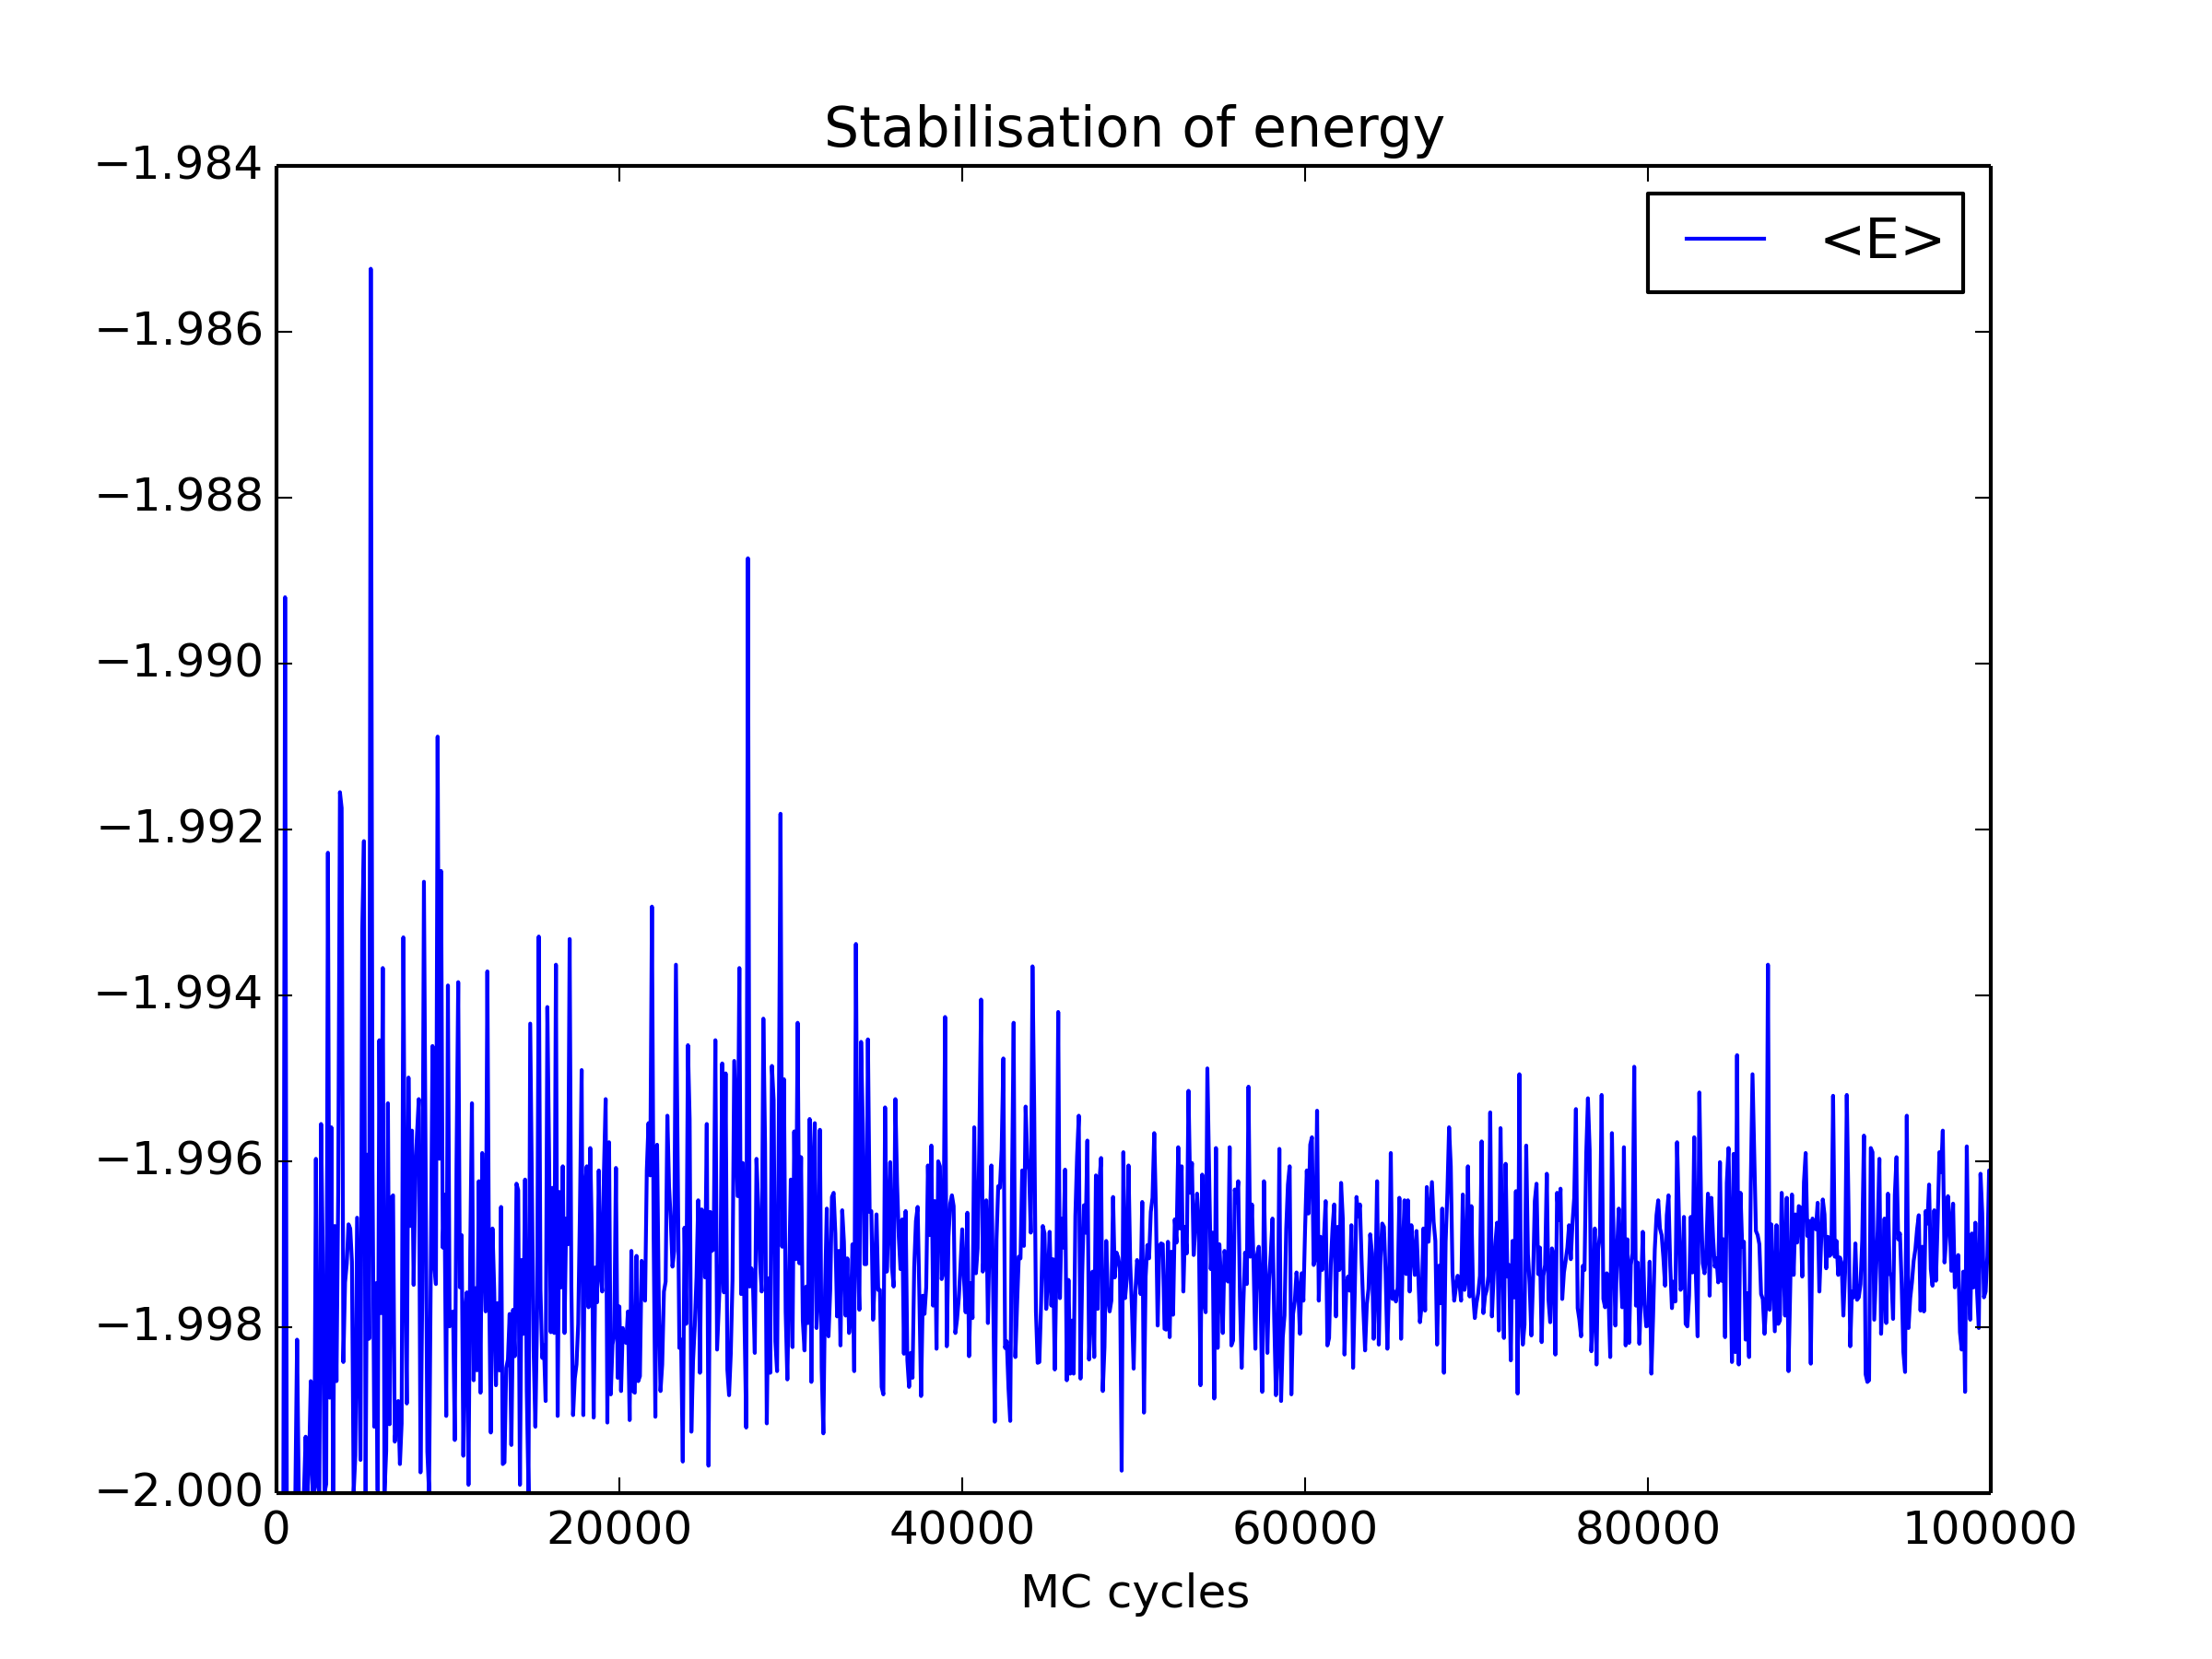
\includegraphics[width=250px]{./plot/L20_1mill.png}
				\caption{Initial matrix with all spins up. }
		\end{subfigure} \hfill %
		\begin{subfigure}{.5\textwidth}
				\centering
				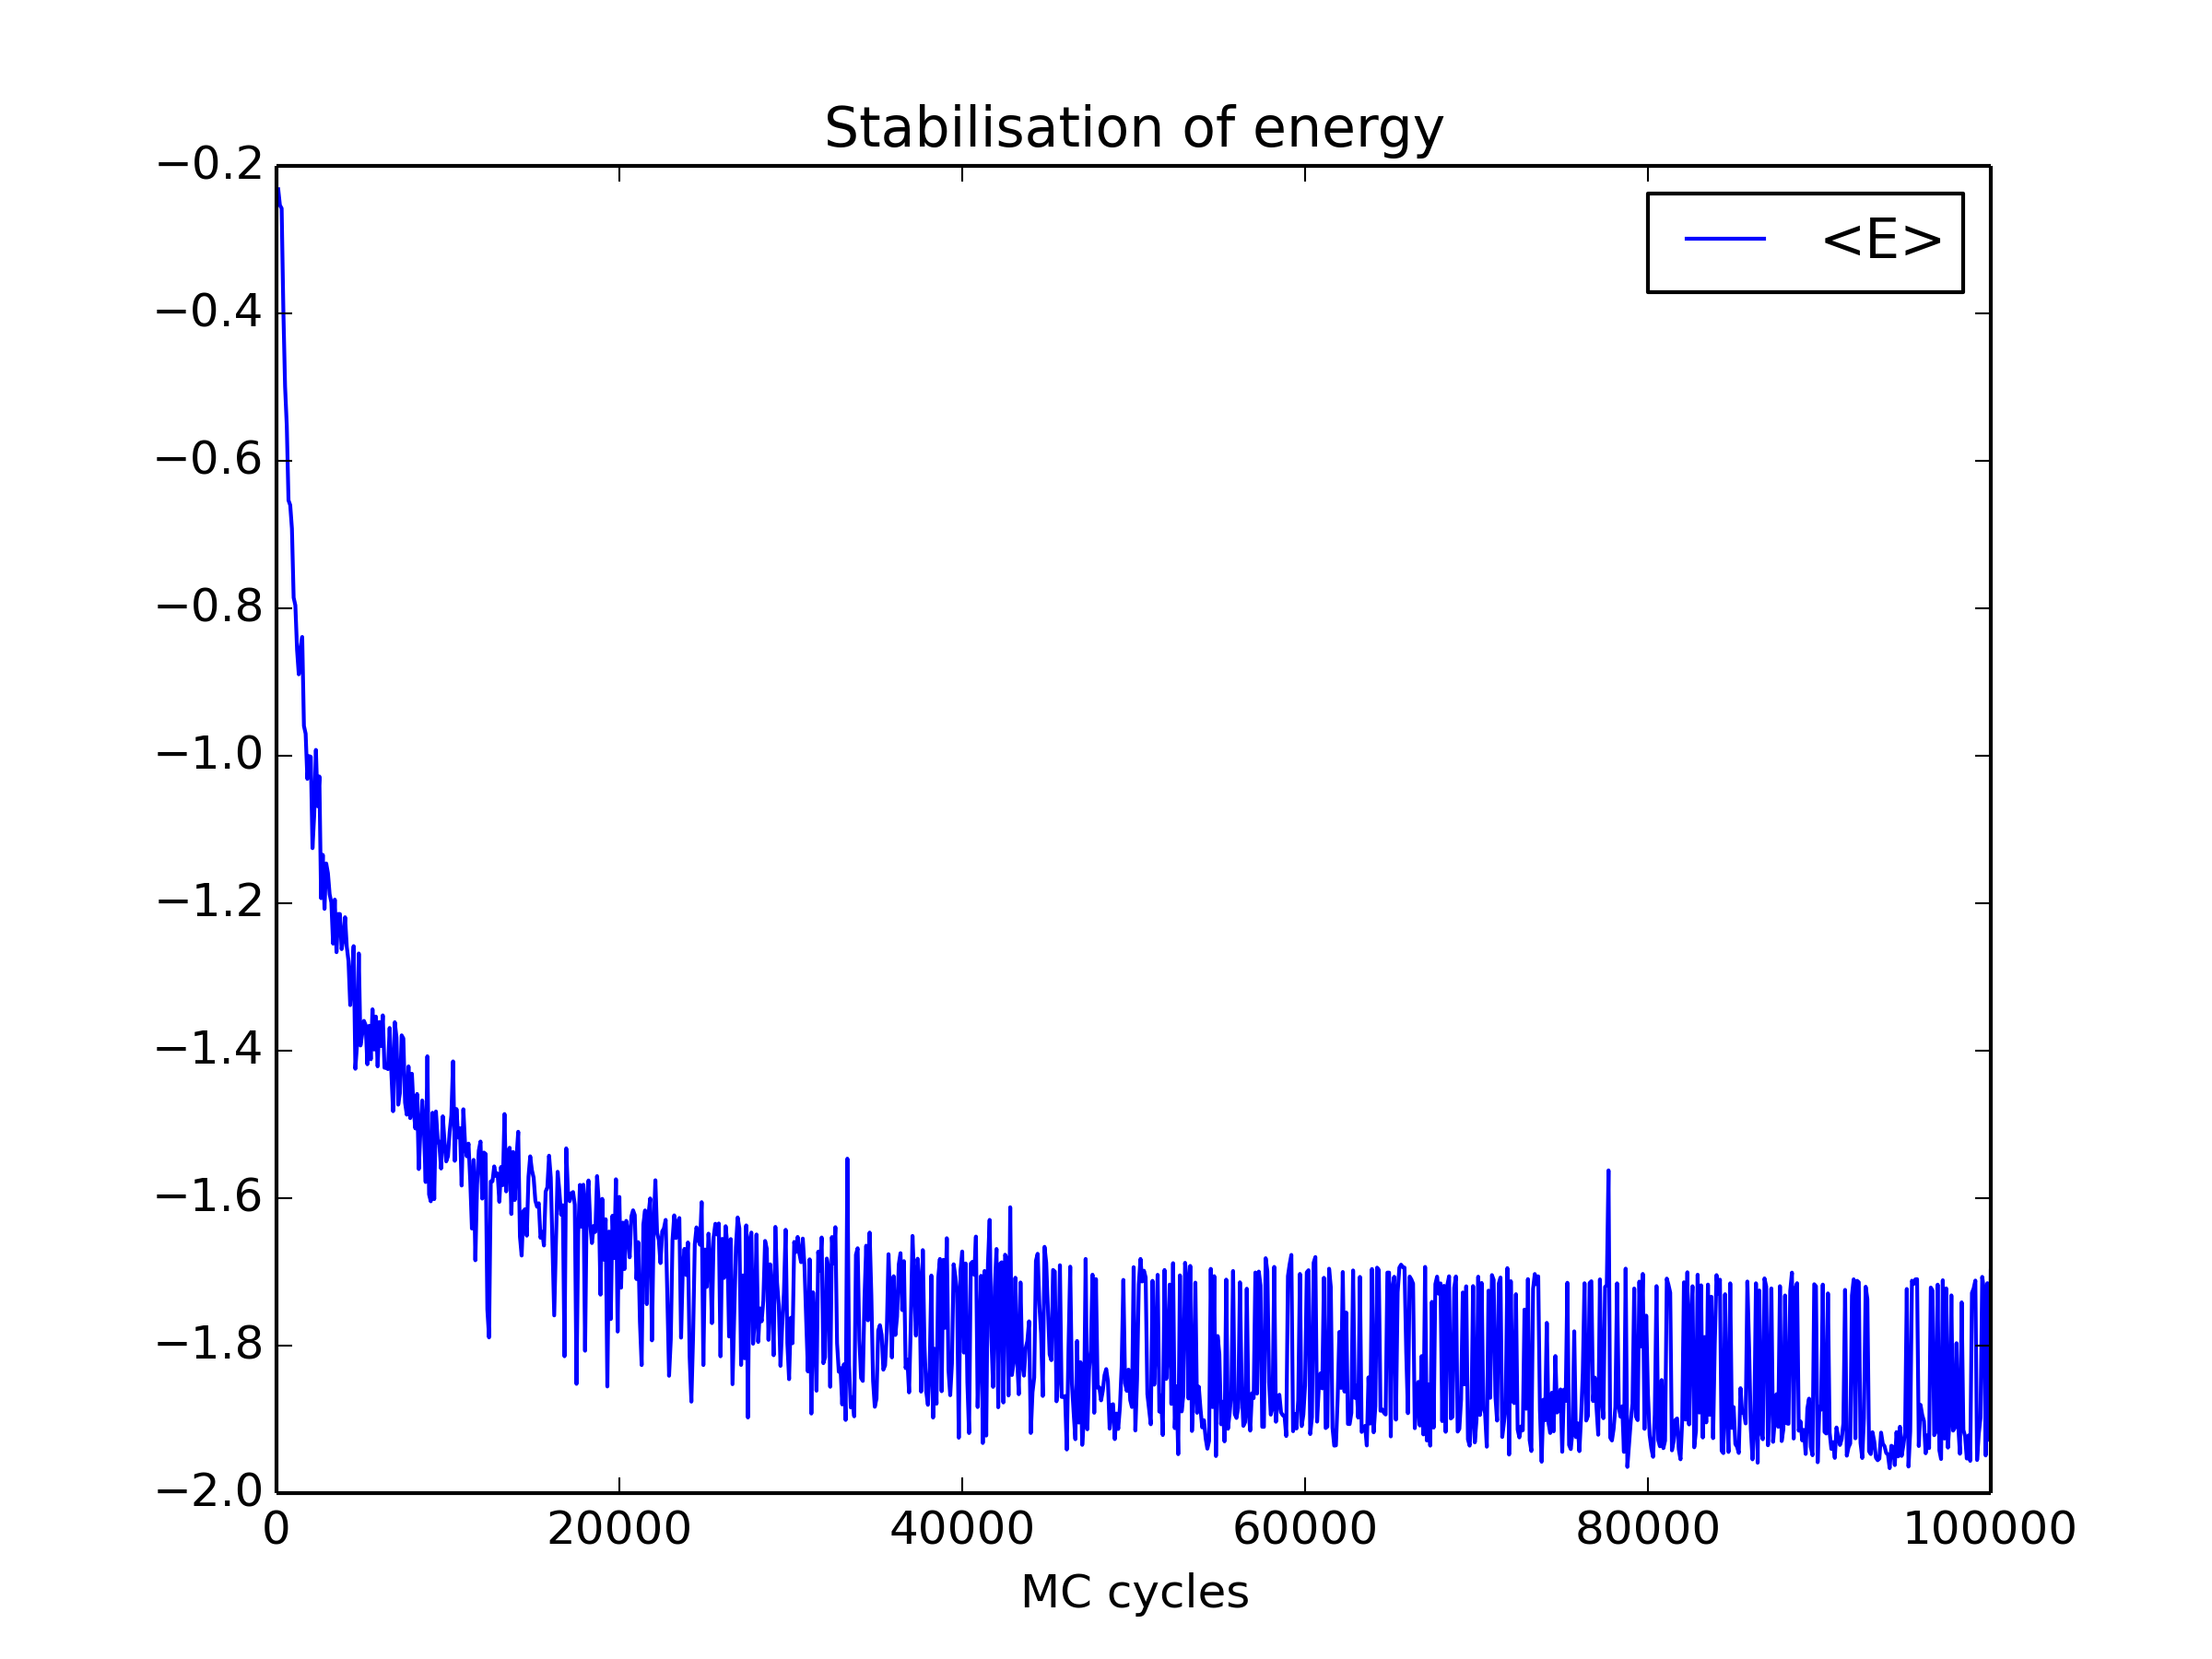
\includegraphics[width=250px]{./plot/random_L20_1mill.png}
				\caption{Initial matrix with random spins.}
		\end{subfigure}\hfill}}
		\caption{: Mean energy plotted against number of Monte Carlo cycles when $T = 1.0$.}
		\label{fig:steady_E}
		\end{figure}

		When we increase the temperature, we see that we need approximately the same number of Monte Carlo cycles, around 50 000, as seen in figure \ref{fig:steady_E_highT}. An estimate for the actual time it takes to reach equilibrium based on the number of Monte Carlo cycles can be made if we assume that one Monte Carlo cycle equals 1 second. The estimated equilibration times can be found in Table \ref{Tab:equilibration_times}.

		\begin{figure}[H]
		\makebox[\textwidth]{\makebox[1.5\textwidth]{%
		\begin{subfigure}{.5\textwidth}
				\centering
				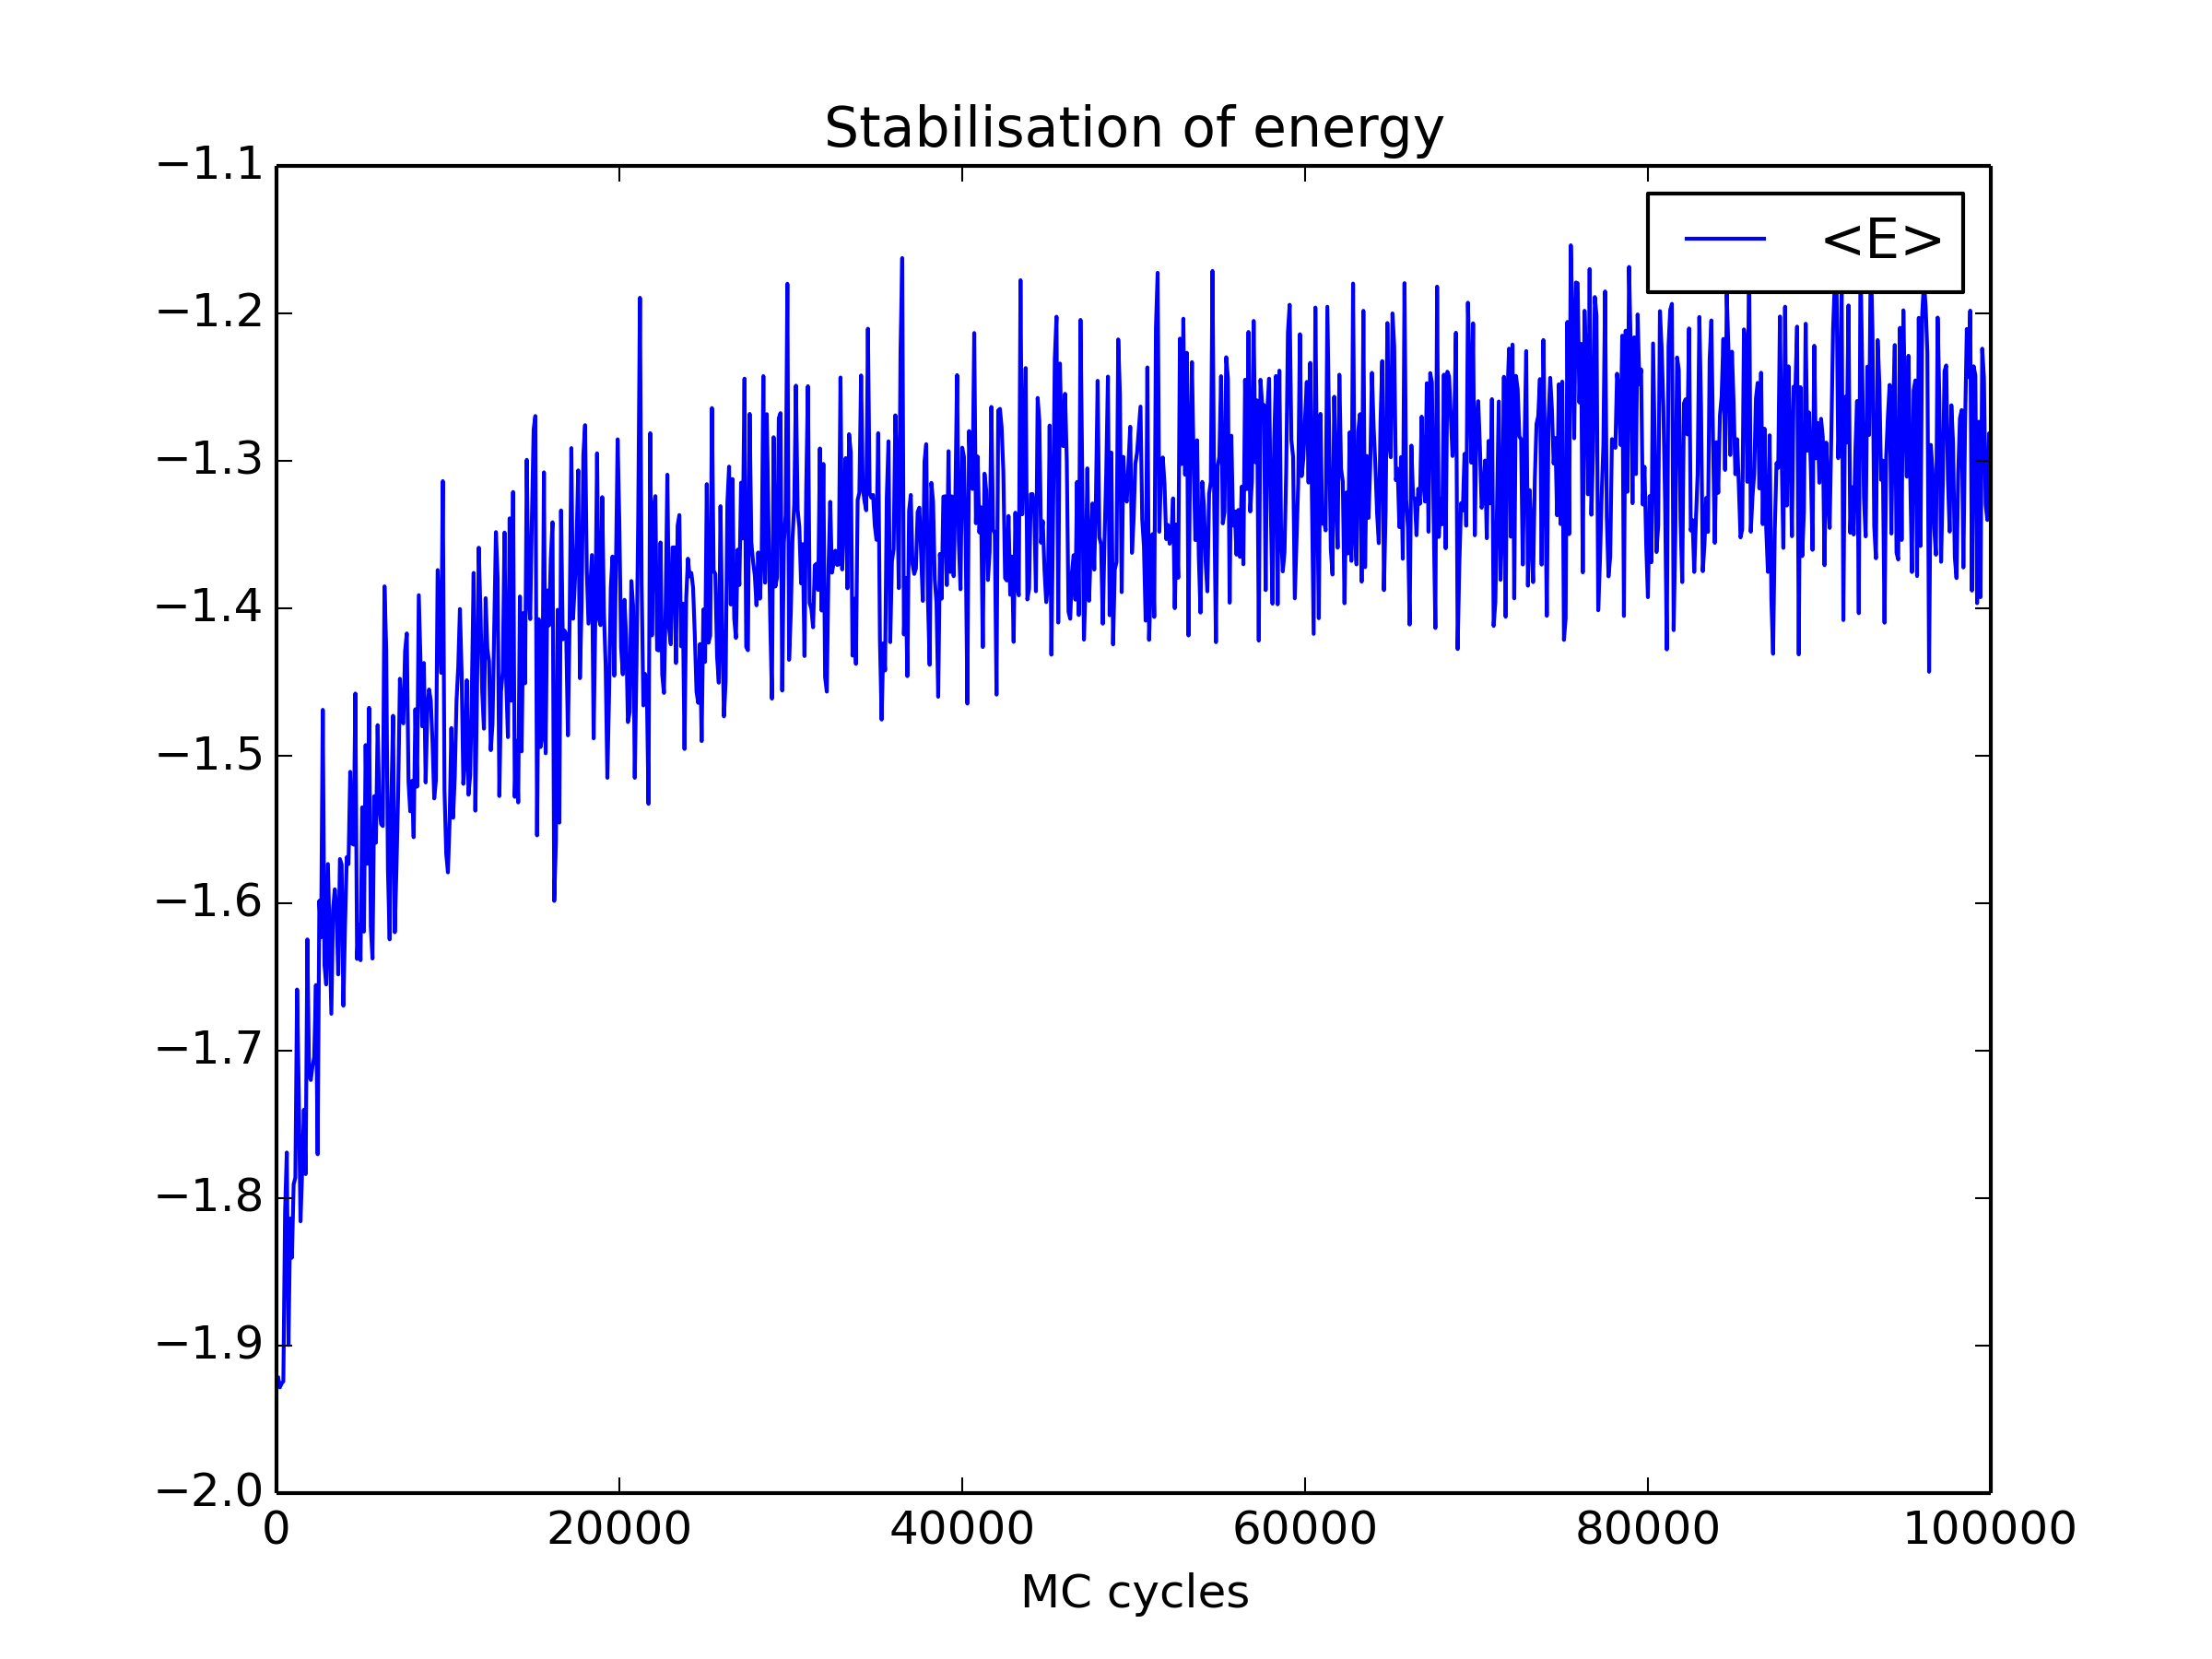
\includegraphics[width=250px]{./plot/L20_1mill_highT.png}
				\caption{Initial matrix with all spins up. }
		\end{subfigure} \hfill %
		\begin{subfigure}{.5\textwidth}
				\centering
				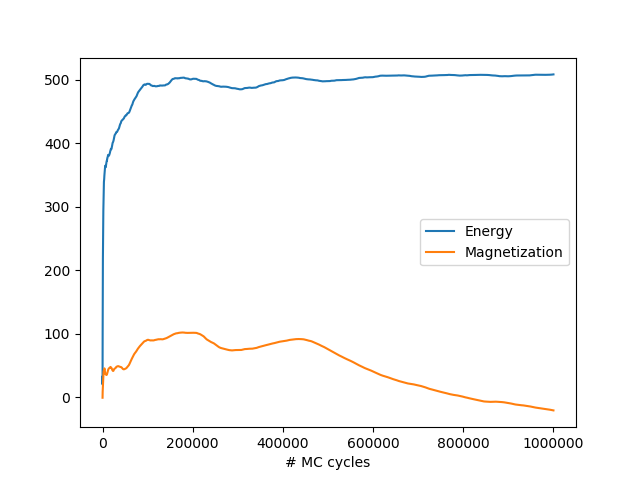
\includegraphics[width=250px]{./plot/random_L20_1mill_highT.png}
				\caption{Initial matrix with random spins.}
		\end{subfigure}\hfill}}
		\caption{: Mean energy plotted against number of Monte Carlo cycles when $T = 2.4$. }
		\label{fig:steady_E_highT}
		\end{figure}

		However, when we perform the same simulation for the magnetisation of the system, we get a different result. In Figure \ref{fig:steady_M} we can see the way the magnetisation varies over MC cycles for $T=1.0$. The magnetisation seems to vary too much to be able to define a reasonable stabilisation point.

		\begin{figure}[H]
		\makebox[\textwidth]{\makebox[1.5\textwidth]{%
			\begin{subfigure}{.5\textwidth}
					\centering
					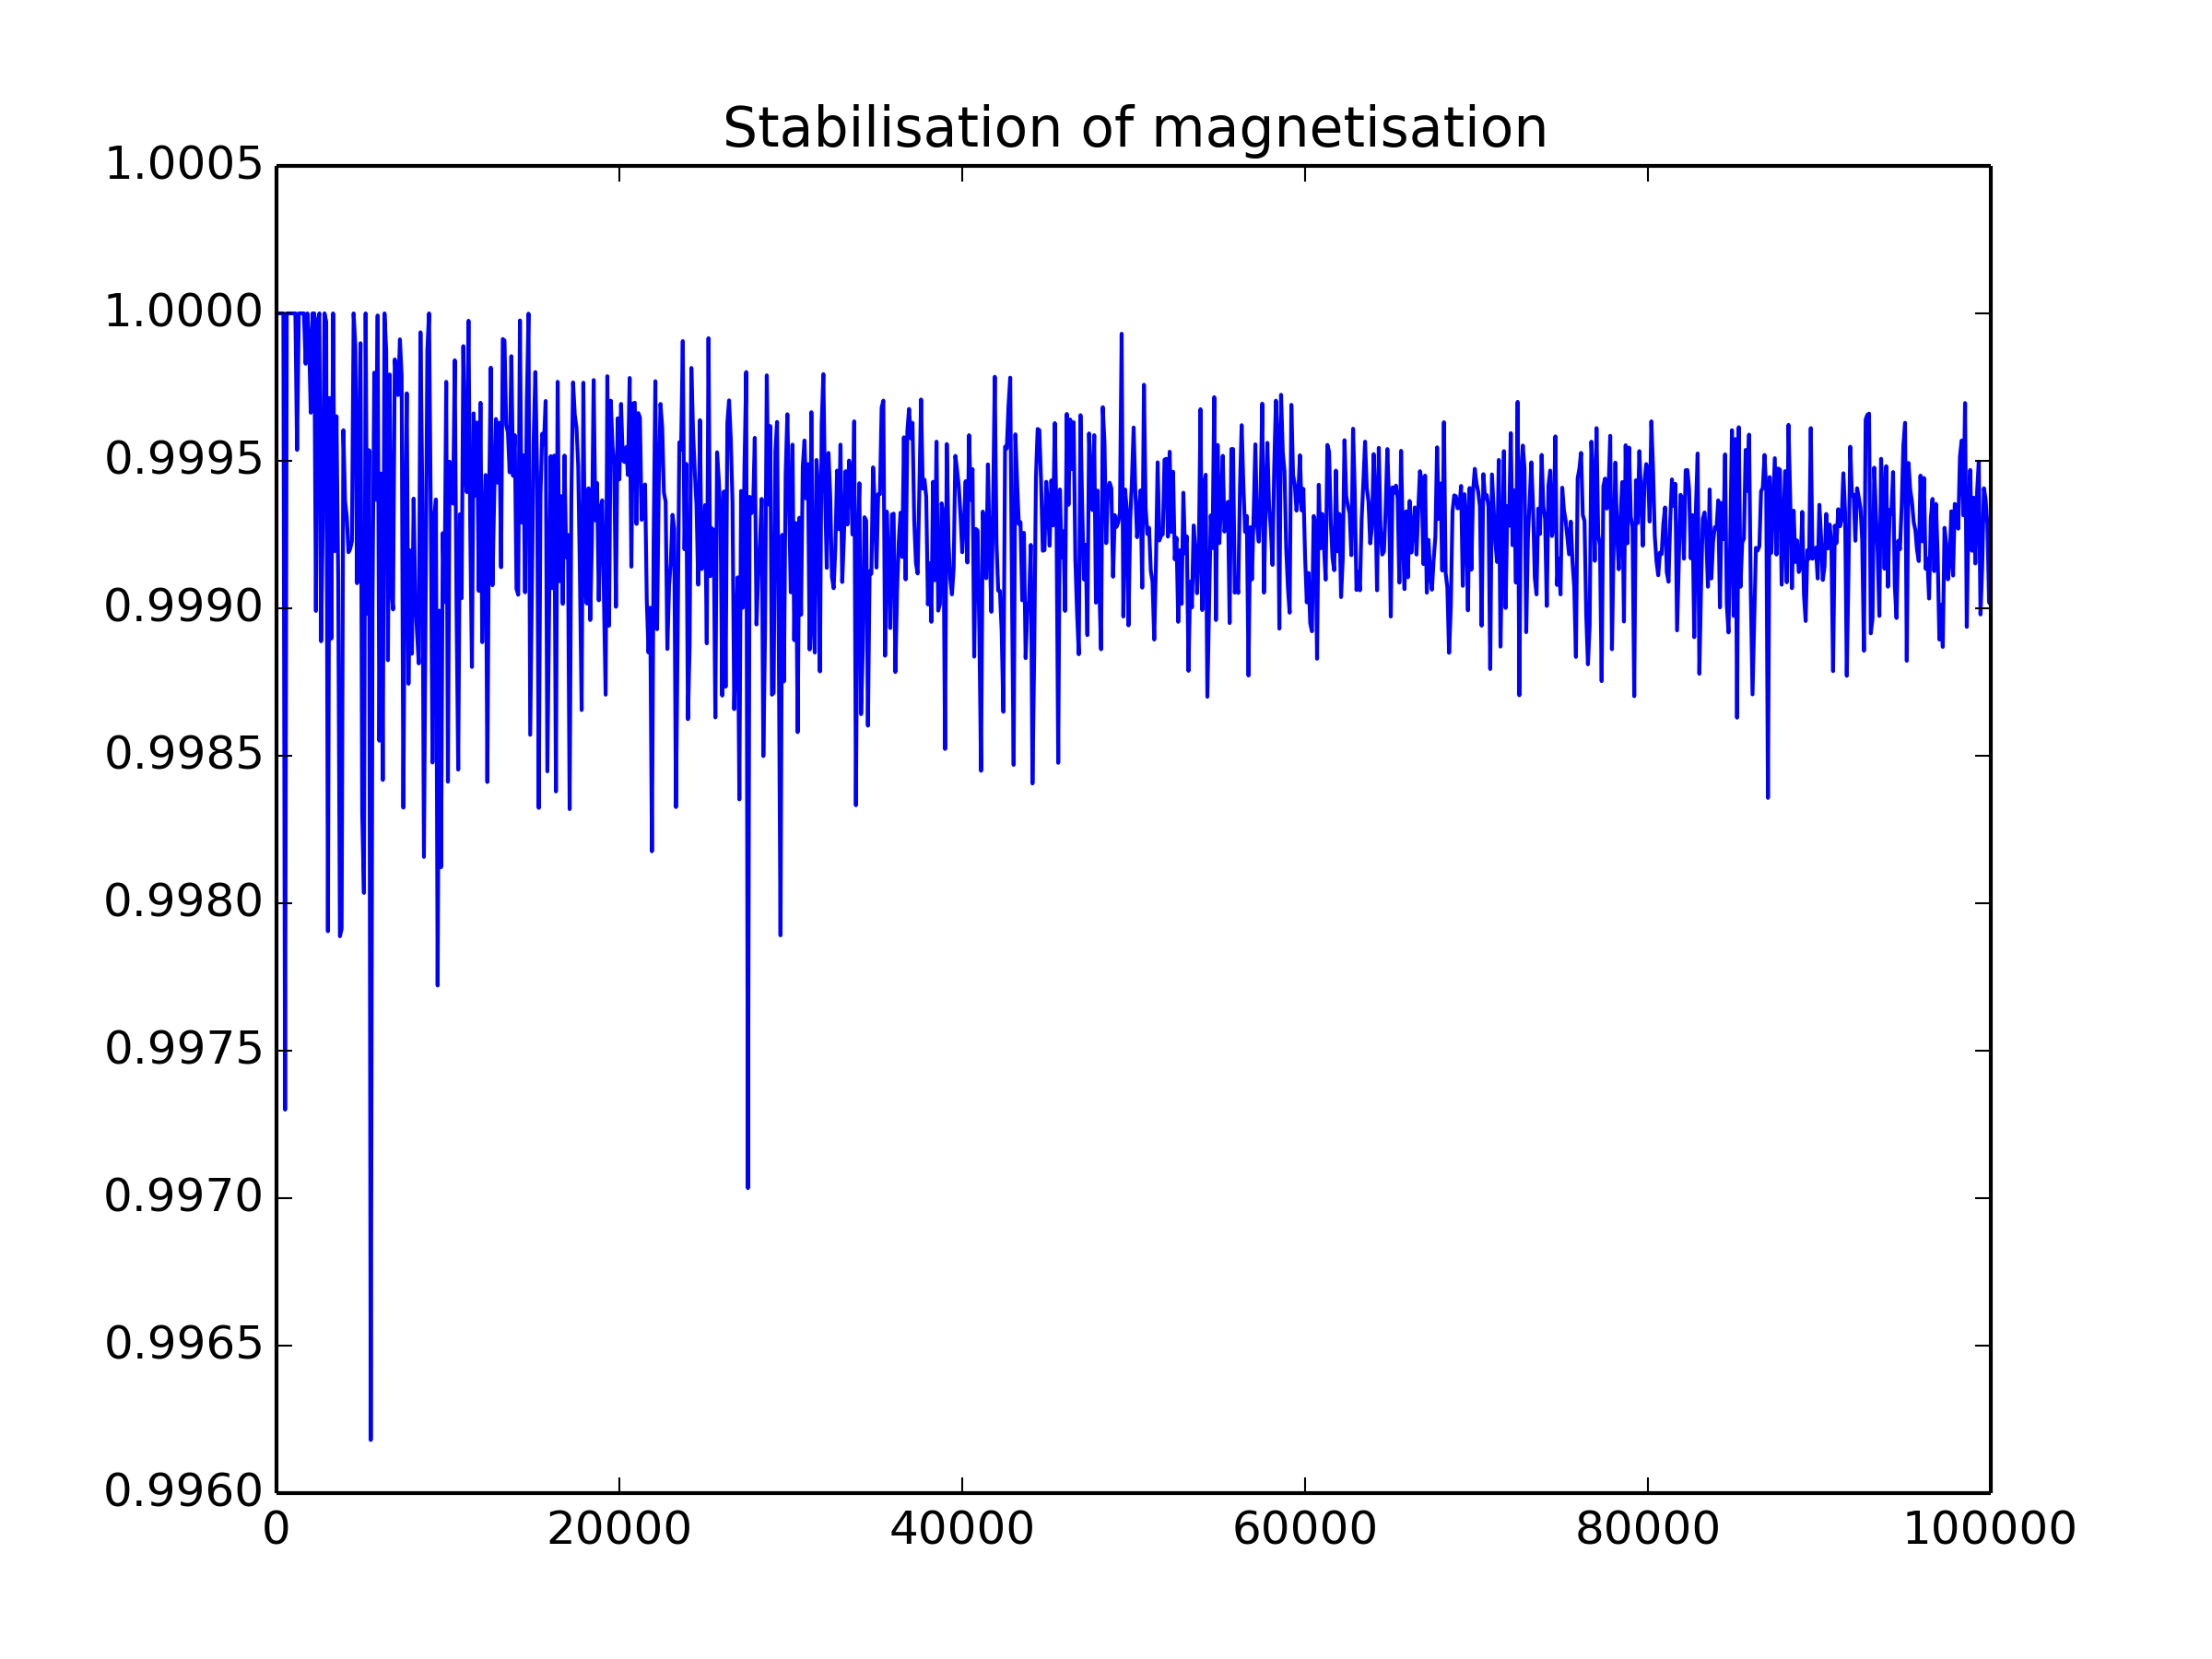
\includegraphics[width=250px]{./plot/M_stabilisation_T=1.png}
					\caption{Initial matrix with all spins up. }
			\end{subfigure} \hfill %
			\begin{subfigure}{.5\textwidth}
					\centering
					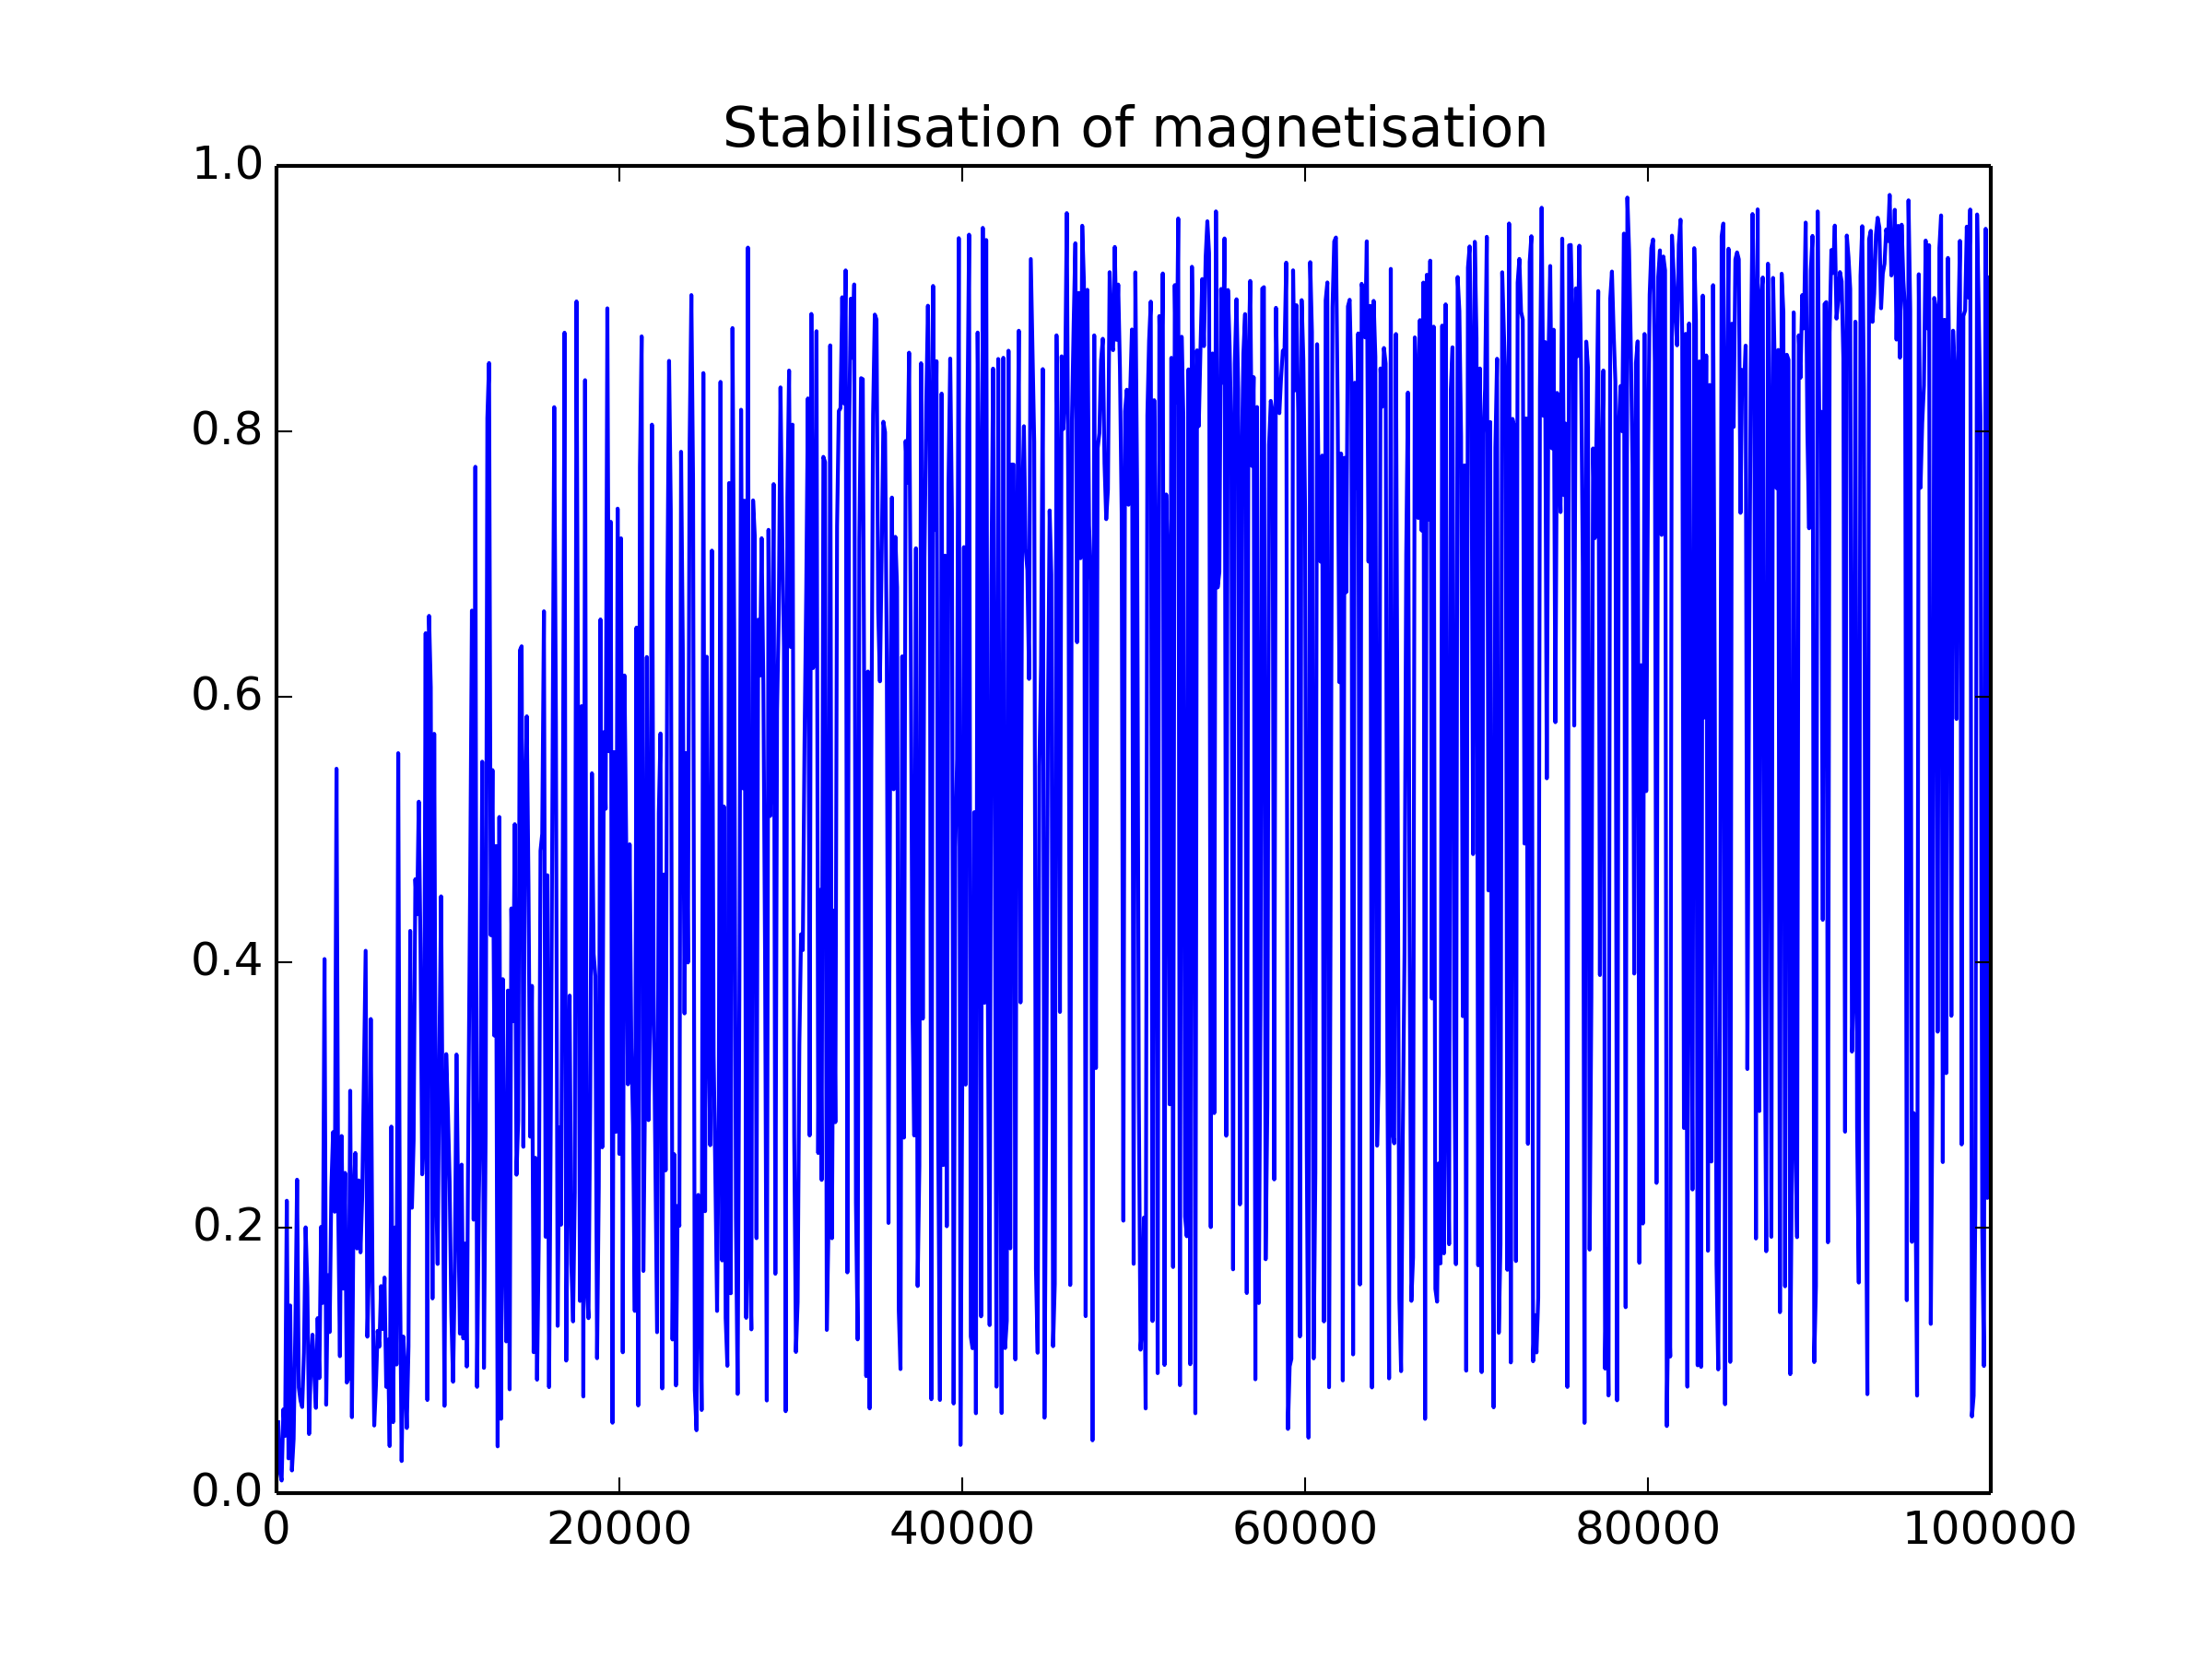
\includegraphics[width=250px]{./plot/M_stabilisation_T=1_rand.png}
					\caption{Initial matrix with random spins.}
			\end{subfigure}\hfill}}
		\caption{: Mean absolute magnetization plotted against number of Monte Carlo cycles when $T = 1$. }
		\label{fig:steady_M}
		\end{figure}

		When the temperature increases it does not get easier to judge whether we get to an equilibrium state or not. This is shown in Figure \ref{fig:steady_M_highT}.

		\begin{figure}[H]
		\makebox[\textwidth]{\makebox[1.5\textwidth]{%
		\begin{subfigure}{.5\textwidth}
				\centering
				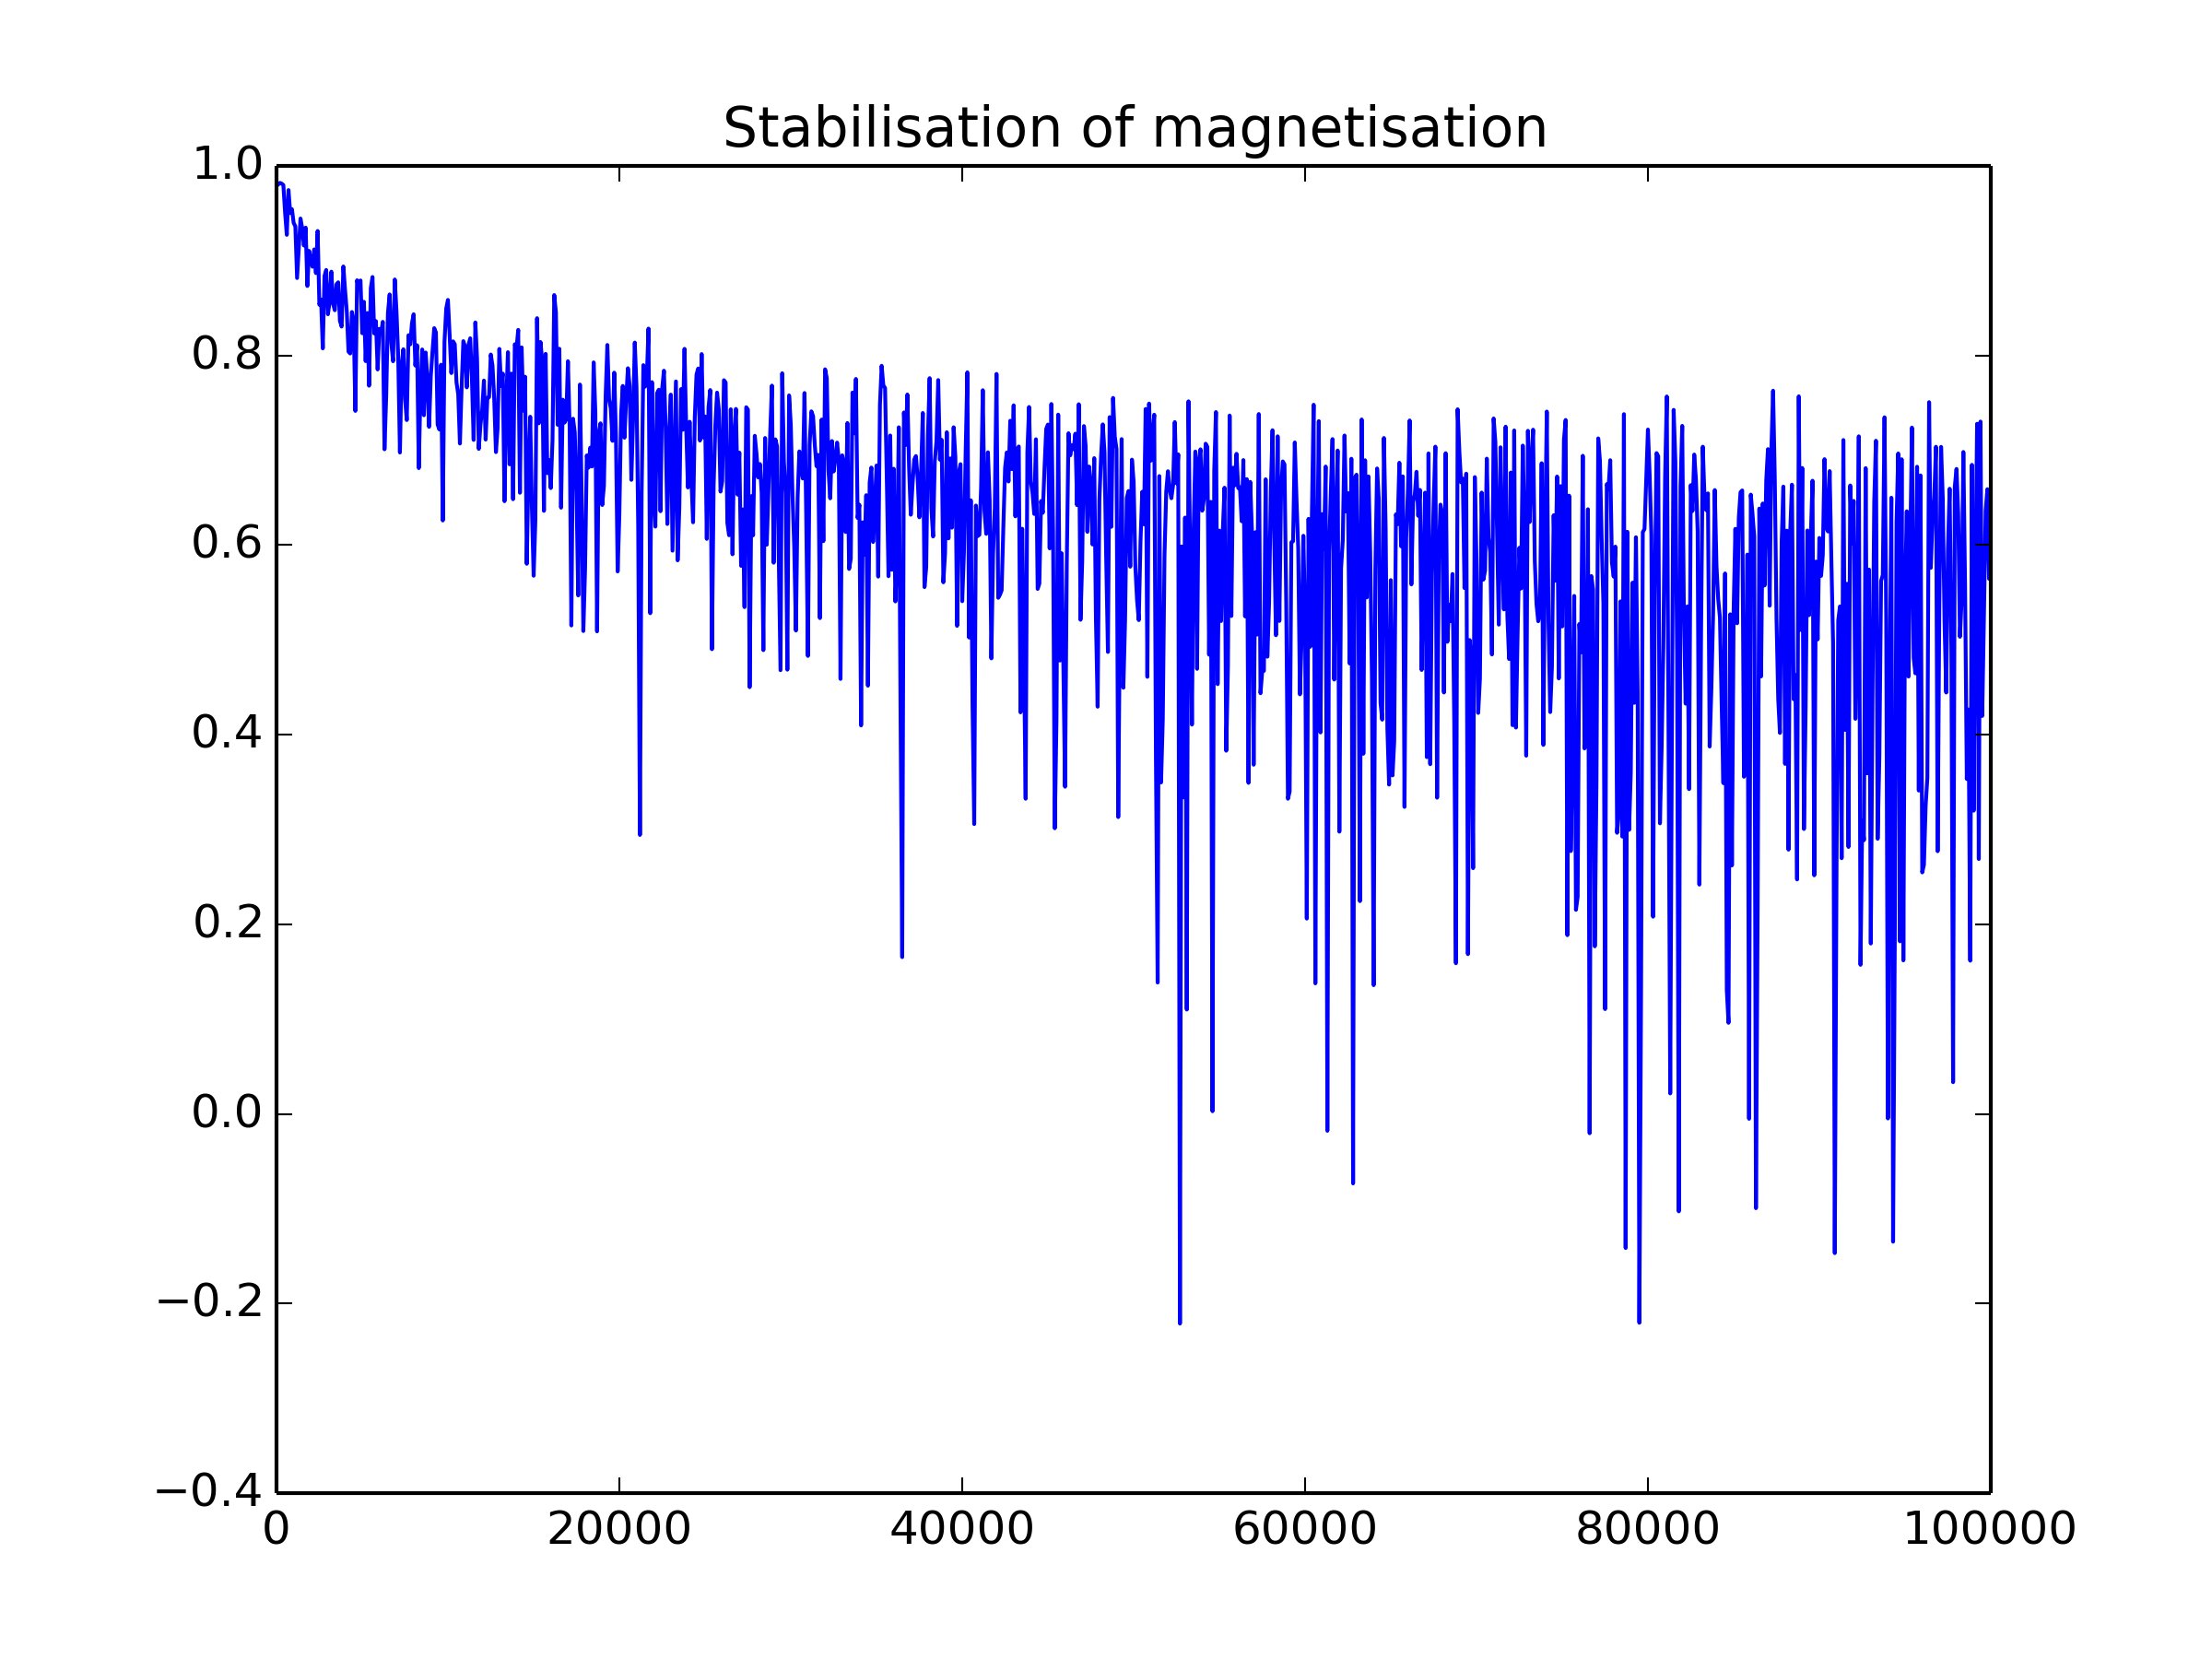
\includegraphics[width=250px]{./plot/M_stabilisation_T=high.png}
				\caption{Initial matrix with all spins up. }
		\end{subfigure} \hfill %
		\begin{subfigure}{.5\textwidth}
				\centering
				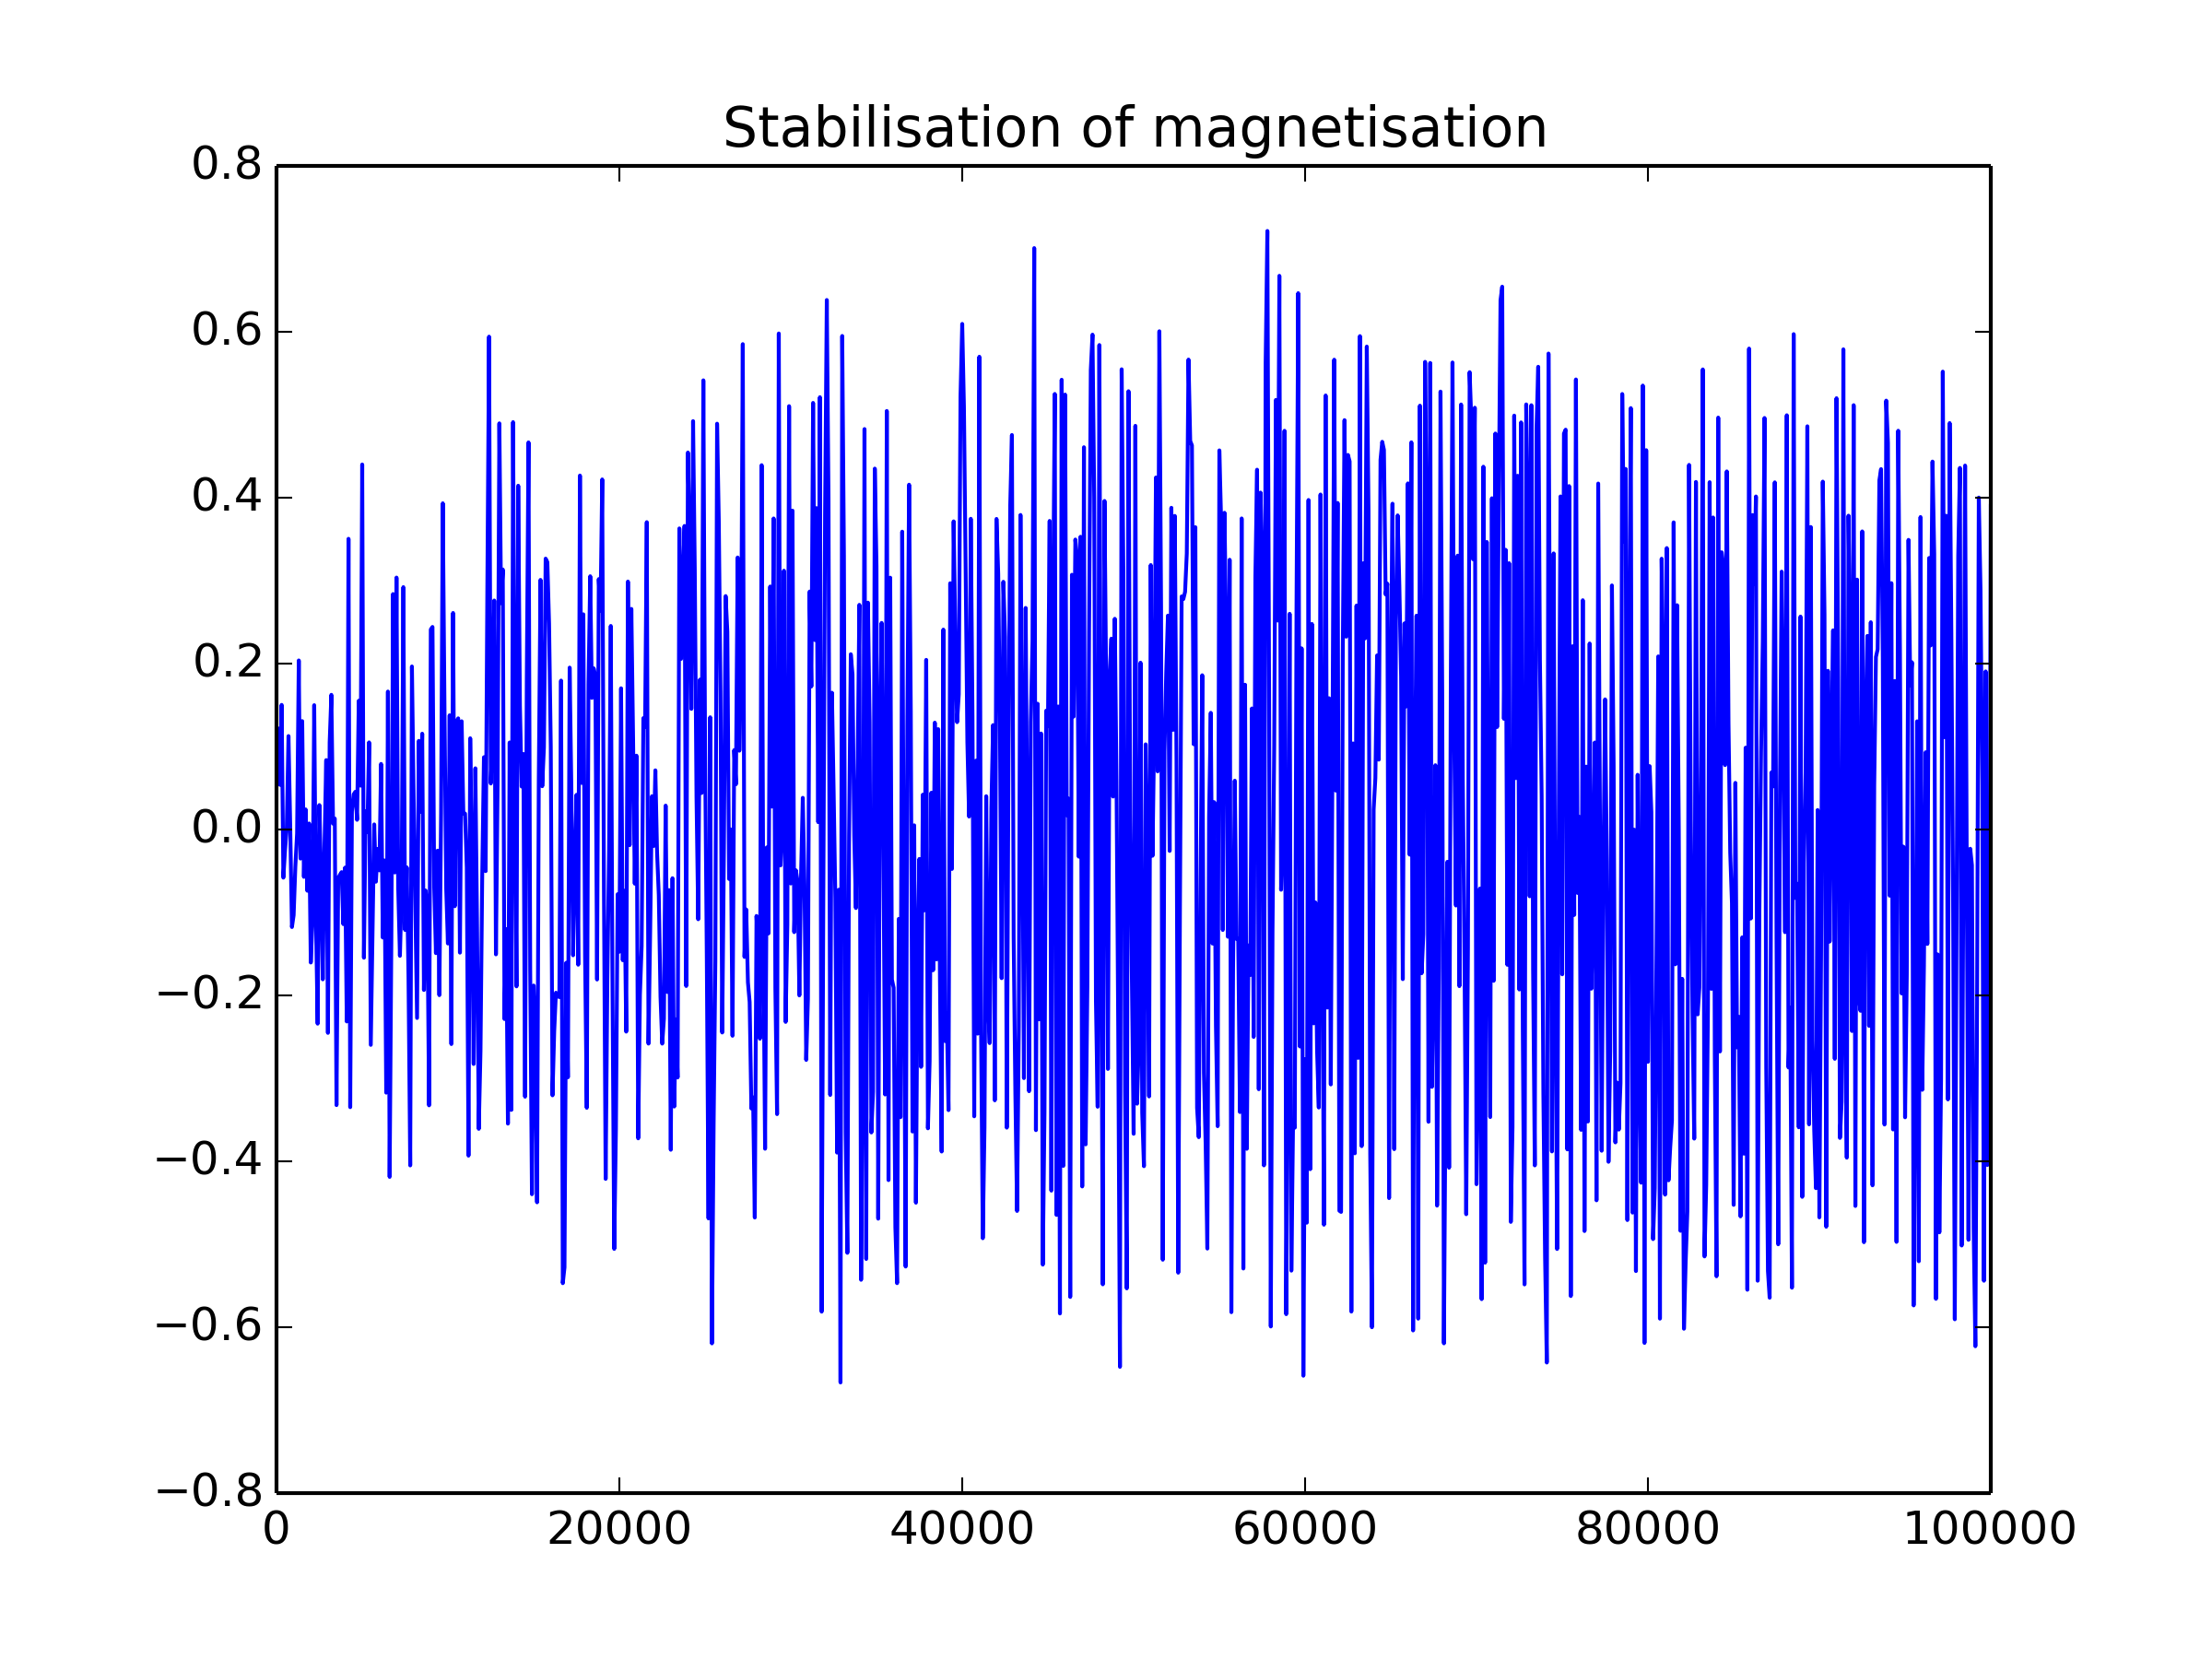
\includegraphics[width=250px]{./plot/M_stabilisation_T=high_rand.png}
				\caption{Initial matrix with random spins.}
		\end{subfigure}\hfill}}
		\caption{: Mean magnetization plotted against number of Monte Carlo cycles when $T = 2.4$. }
		\label{fig:steady_M_highT}
		\end{figure}

		Because it is impossible to decide when the magnetisation stabilizes, we define the point where the system reaches equilibrium to be when the energy stabilizes.
		The estimation of when the system reaches equilibrium for the different initial conditions is found in the following table, \ref{Tab:equilibration_times}.

		{\renewcommand{\arraystretch}{1.5}
		\begin{table}[h!]
			\caption{: Estimated equilibration times.}
				\label{Tab:equilibration_times}
				\centering
			\begin{tabular}{c c c}
					Temperature & Matrix & Equilibration time (minutes)\\
					\hline
					$1.0$ & Random spins & 667 \\
					$1.0$ & All spins up & 667 \\
					$2.4$ & Random spins & 883 \\
					$2.4$ & All spins up & 883 \\
				\hline
			\end{tabular}
		\end{table}

		Figure \ref{fig:flips} and Figure \ref{fig:flips_random} show plots of the total number of accepted configurations as function of the total number of Monte Carlo cycles for respectively an initial matrix with all spins up and an initial matrix with random spins. It is worth mentioning that these plots represent how many flips that have been accepted in the entire lattice per Monte Carlo cycle. Therefore the values are sub zero.

		\begin{figure}[H]
		\makebox[\textwidth]{\makebox[1.5\textwidth]{%
		\begin{subfigure}{.5\textwidth}
				\centering
				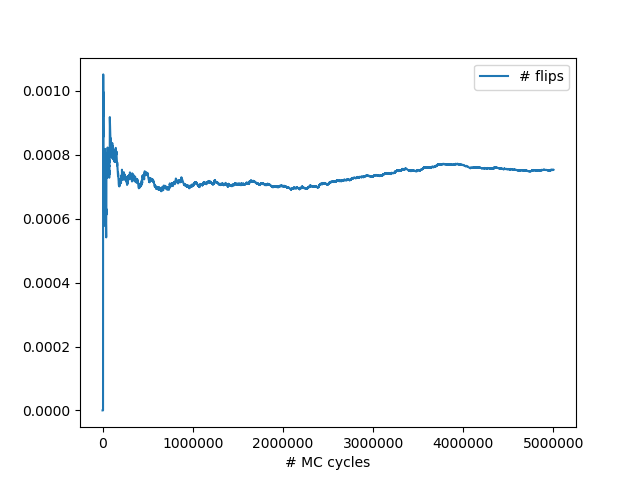
\includegraphics[width=250px]{./plot/number_of_flips.png}
				\caption{T = 1.0}
		\end{subfigure} \hfill %
		\begin{subfigure}{.5\textwidth}
				\centering
				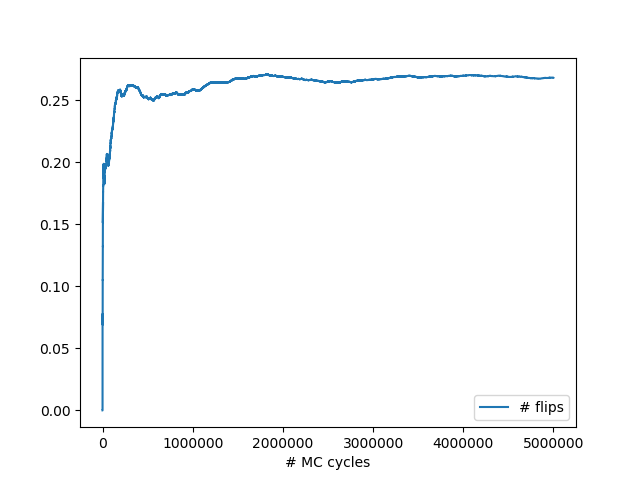
\includegraphics[width=250px]{./plot/number_of_flips_highT.png}
				\caption{T = 2.4}
		\end{subfigure}\hfill}}
		\caption{: Total number of accepted spin configuration as a function of Monte Carlo cycles, for an initial matrix with all spins up. }
		\label{fig:flips}
		\end{figure}

		\begin{figure}[H]
		\makebox[\textwidth]{\makebox[1.5\textwidth]{%
		\begin{subfigure}{.5\textwidth}
				\centering
				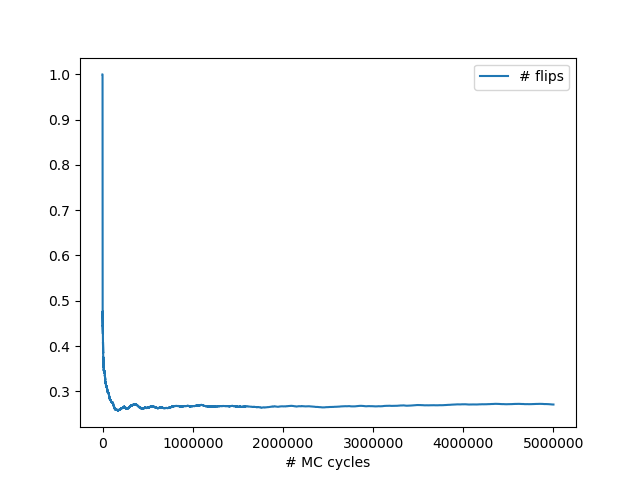
\includegraphics[width=250px]{./plot/random_number_of_flips.png}
				\caption{T = 1.0}
		\end{subfigure} \hfill %
		\begin{subfigure}{.5\textwidth}
				\centering
				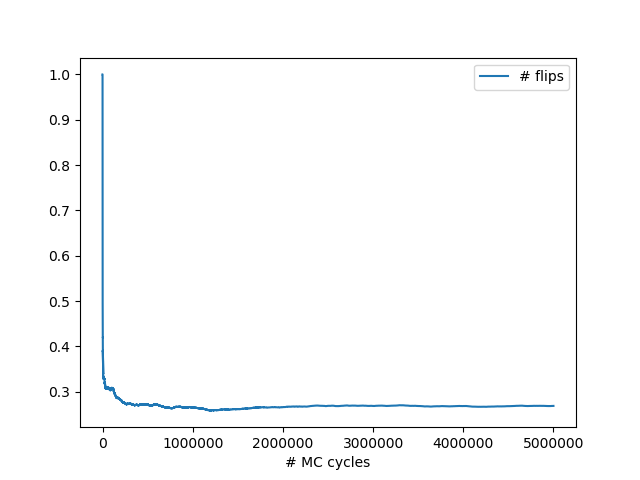
\includegraphics[width=250px]{./plot/random_number_of_flips_highT.png}
				\caption{T = 2.4}
		\end{subfigure}\hfill}}
		\caption{: Total number of accepted spin configuration as a function of Monte Carlo cycles, for an initial matrix with random spins. }
		\label{fig:flips_random}
		\end{figure}
\newpage
	\subsection{Probability Distribution}
		% d)
		The probability distribution of the energy for $T = 1.0$ and $T = 2.4$ is shown in figure \ref{fig:probability}

		\begin{figure}[H]
		\makebox[\textwidth]{\makebox[1.5\textwidth]{%
		\begin{subfigure}{.5\textwidth}
				\centering
				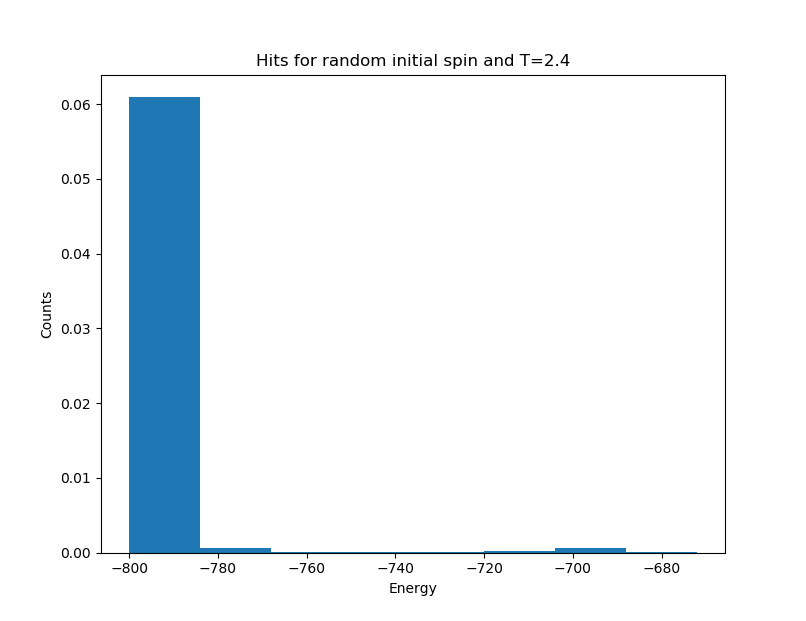
\includegraphics[width=250px]{./plot/histogram_random_lowT.png}
				\caption{$T = 1.0$}
		\end{subfigure} \hfill %
		\begin{subfigure}{.5\textwidth}
				\centering
				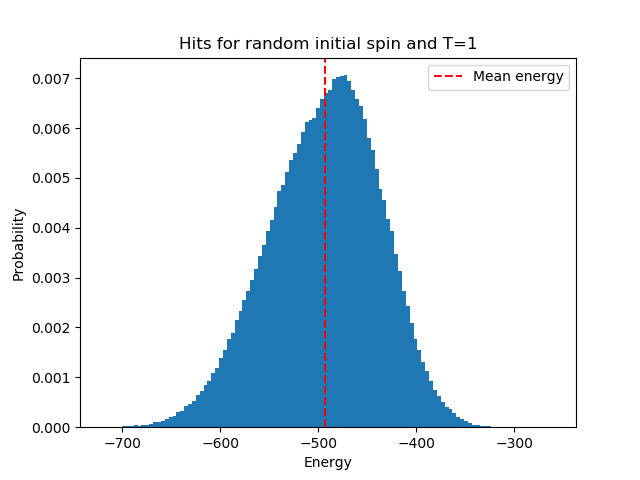
\includegraphics[width=300px]{./plot/histogram_random_highT.png}
				\caption{$T = 2.4$}
		\end{subfigure}\hfill}}
		\caption{: Probability distribution for counted energies.}
		\label{fig:probability}
		\end{figure}

	\subsection{Phase Transitions}
		During our tests runs with the Ising model with various lattice sizes and MC cycles, we gathered information about the time it takes to perform our calculations, which we used to estimate how many cycles we can perform for each of our required temperature steps within a reasonable computation duration.

		Running our model for one million Monte Carlo cycles and 20 temperature steps on the same computer using one core takes 4.93 minutes, while using four cores takes 1.59 minutes. This shows that parallelization gives us a significant speed-up for our calculations.

		We landed on having 12 temperature steps in the range $T = [2.0, 2.3]$, because we had four cores available for computations, and the way we parallelizes meant each core then had 3 temperature steps to compute, with a total of $10^8$ Monte Carlo cycles each. Running this calculation on a four core 2,5 GHz computer took $131.7$ minutes to complete.

		In Figure \ref{fig:mean_E_M} and \ref{fig:heat_susc} we have plotted the mean energy, the mean magnetisation, the heat capacity and the susceptibility as a function of T for different lattice sizes, L = 40, L = 60, L = 80 and L = 100. From these simulations and by using Equation \ref{eq:TC} we have estimated the critical temperature, $T_C$ for the system. The critical temperature for the different lattice sizes are shown in Table \ref{Tab:TC}

		{\renewcommand{\arraystretch}{1.5}
		\begin{table}[h!]
			\caption{: Critical temperatures for different lattice sizes.}
				\label{Tab:TC}
				\centering
			\begin{tabular}{c c}
					Lattice & Critical Temperature\\
					\hline
					L = 40 & 2.31 \\
					L = 60 & 2.35 \\
					L = 80 & 2.35 \\
					L = 100	& 2.44 \\
				\hline
			\end{tabular}
		\end{table}

		We then use Equation \ref{eq:a} to find $T_C(L=\infty)$ from \ref{eq:TC}. We use the critical temperature for L = 80 and L = 100, which determines that $a = -36$, resulting in $T_C(L=\infty) = 2.78$.


		\begin{figure}[H]
		\makebox[\textwidth]{\makebox[1.5\textwidth]{%
		\begin{subfigure}{.5\textwidth}
				\centering
				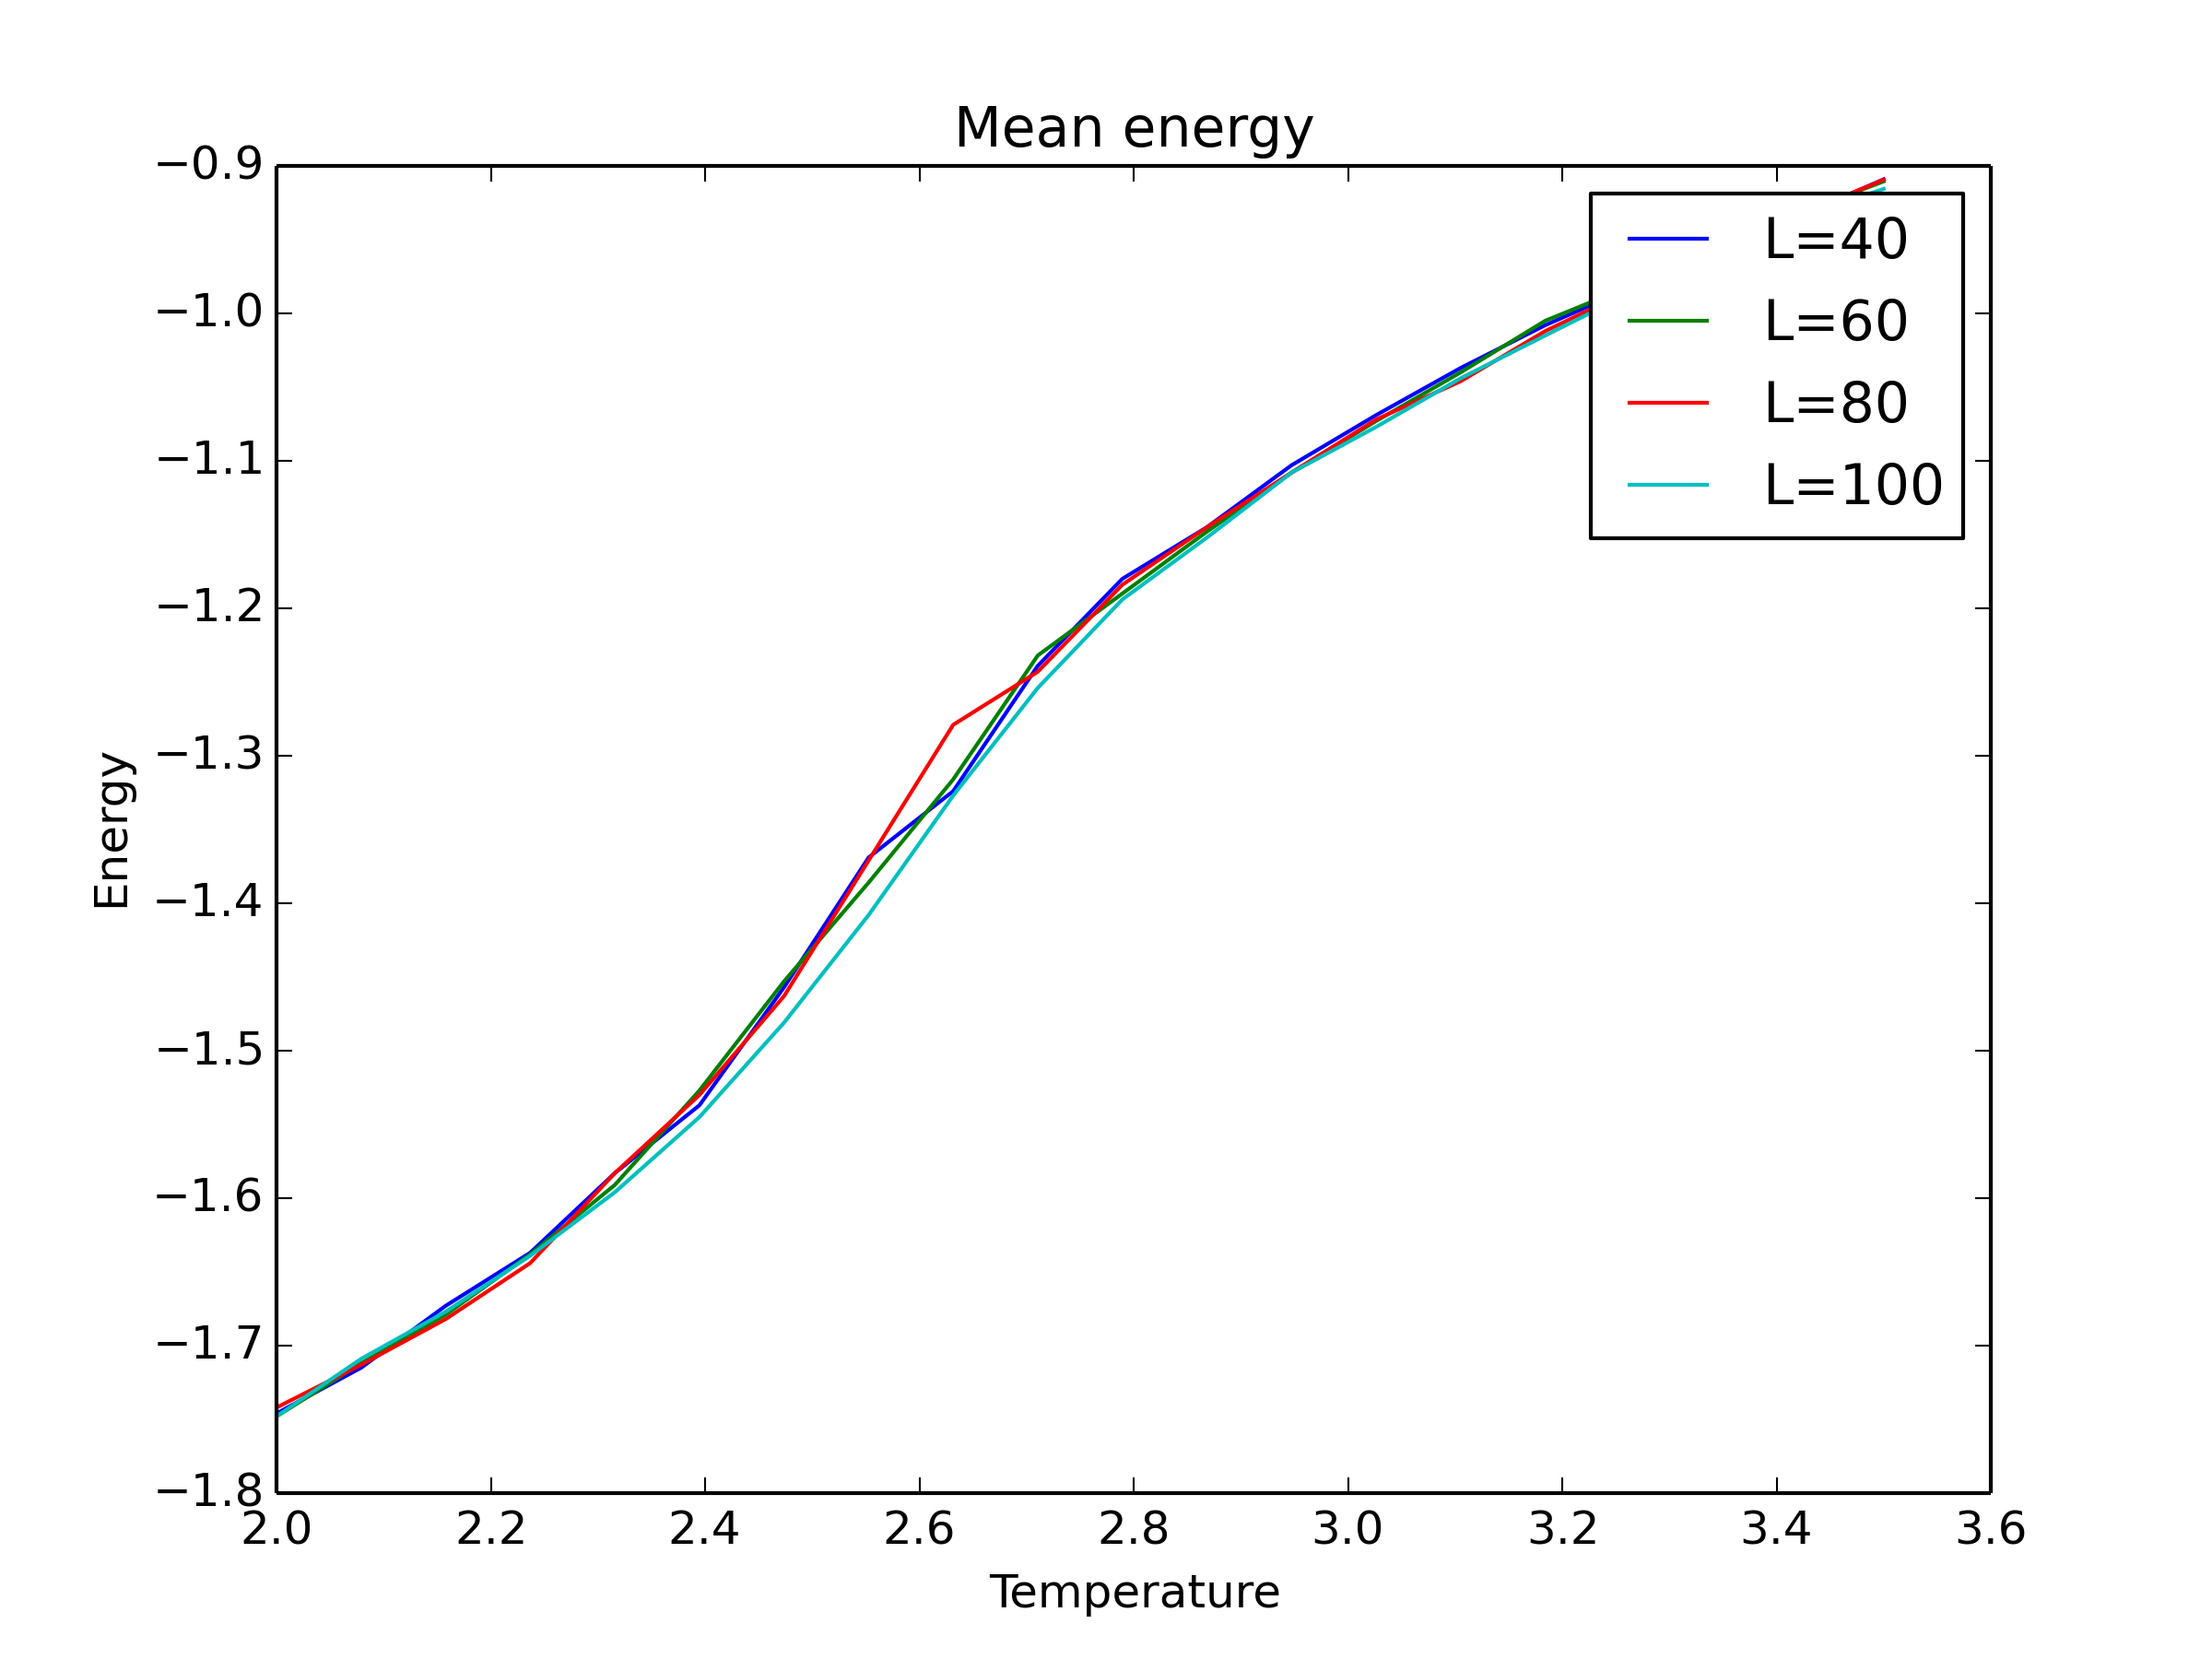
\includegraphics[width=250px]{./Plotting/Mean_E.png}
				\caption{Mean Energy }
		\end{subfigure} \hfill %
		\begin{subfigure}{.5\textwidth}
				\centering
				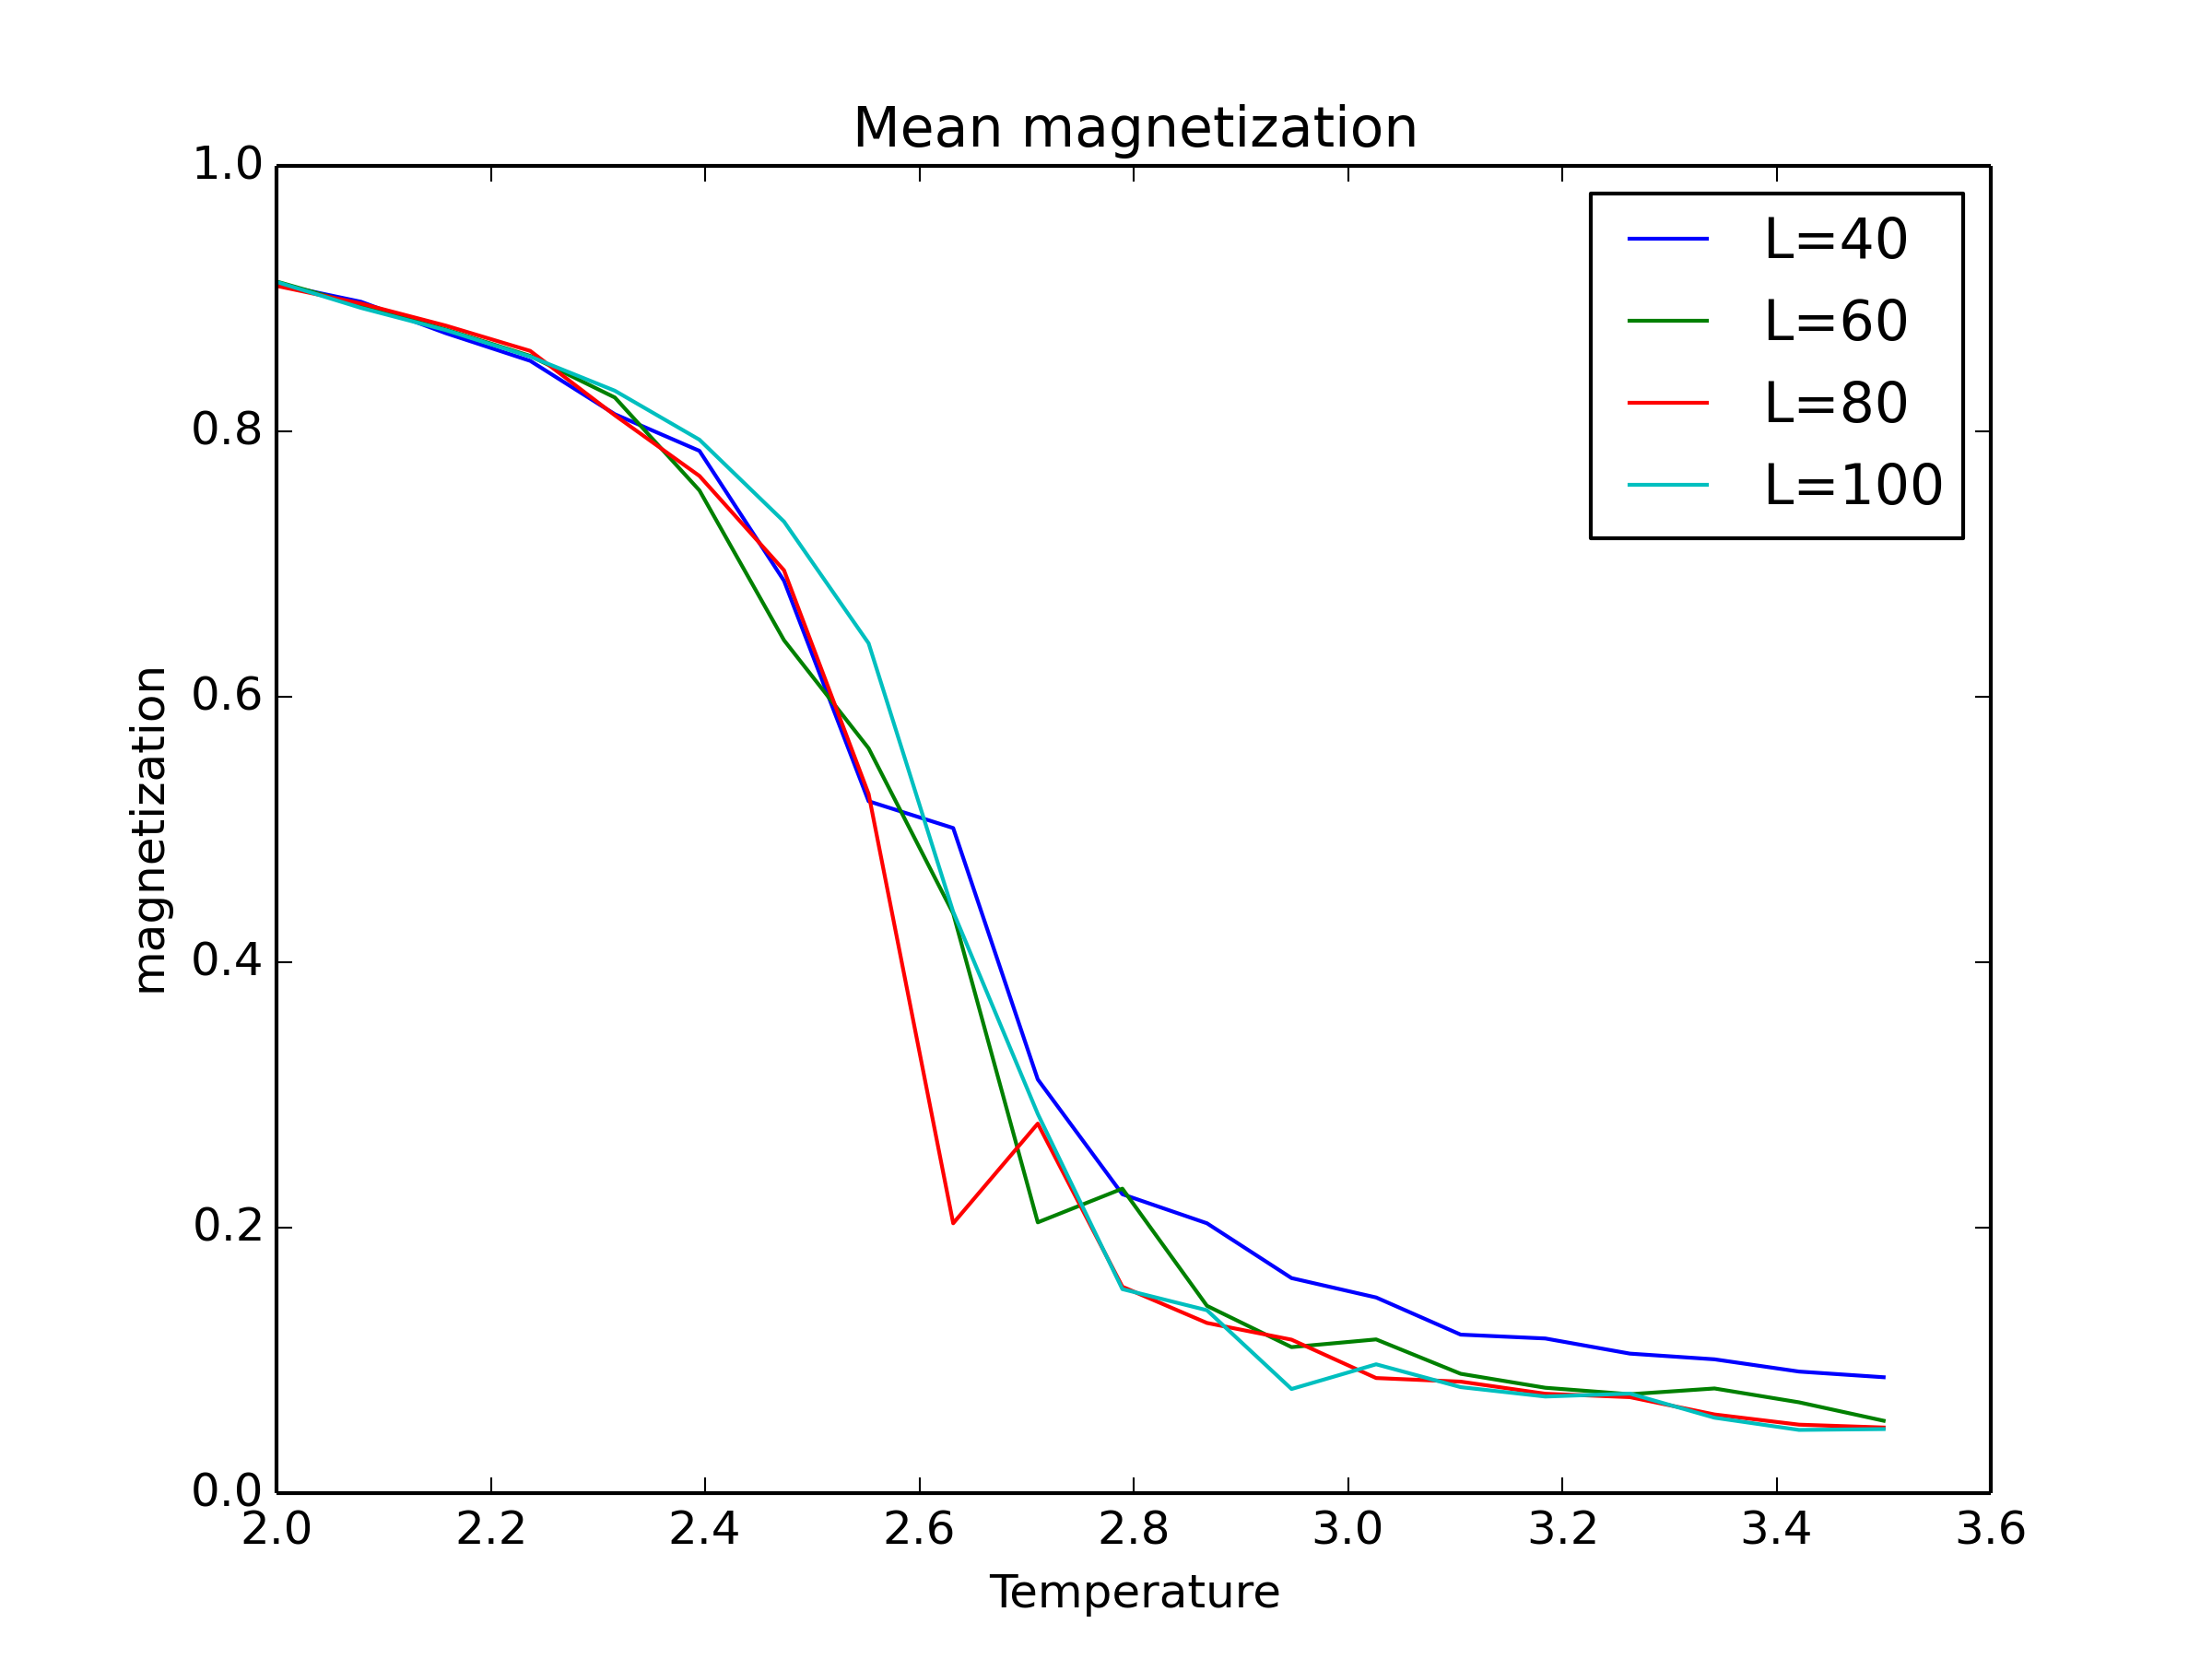
\includegraphics[width=250px]{./Plotting/Mean_M.png}
				\caption{Mean Magnetization.}
		\end{subfigure}\hfill}}
		\caption{: Energy and Magnetization as functions of temperature for different lattice sizes, L.}
		\label{fig:mean_E_M}
		\end{figure}


		\begin{figure}[H]
		\makebox[\textwidth]{\makebox[1.5\textwidth]{%
		\begin{subfigure}{.5\textwidth}
				\centering
				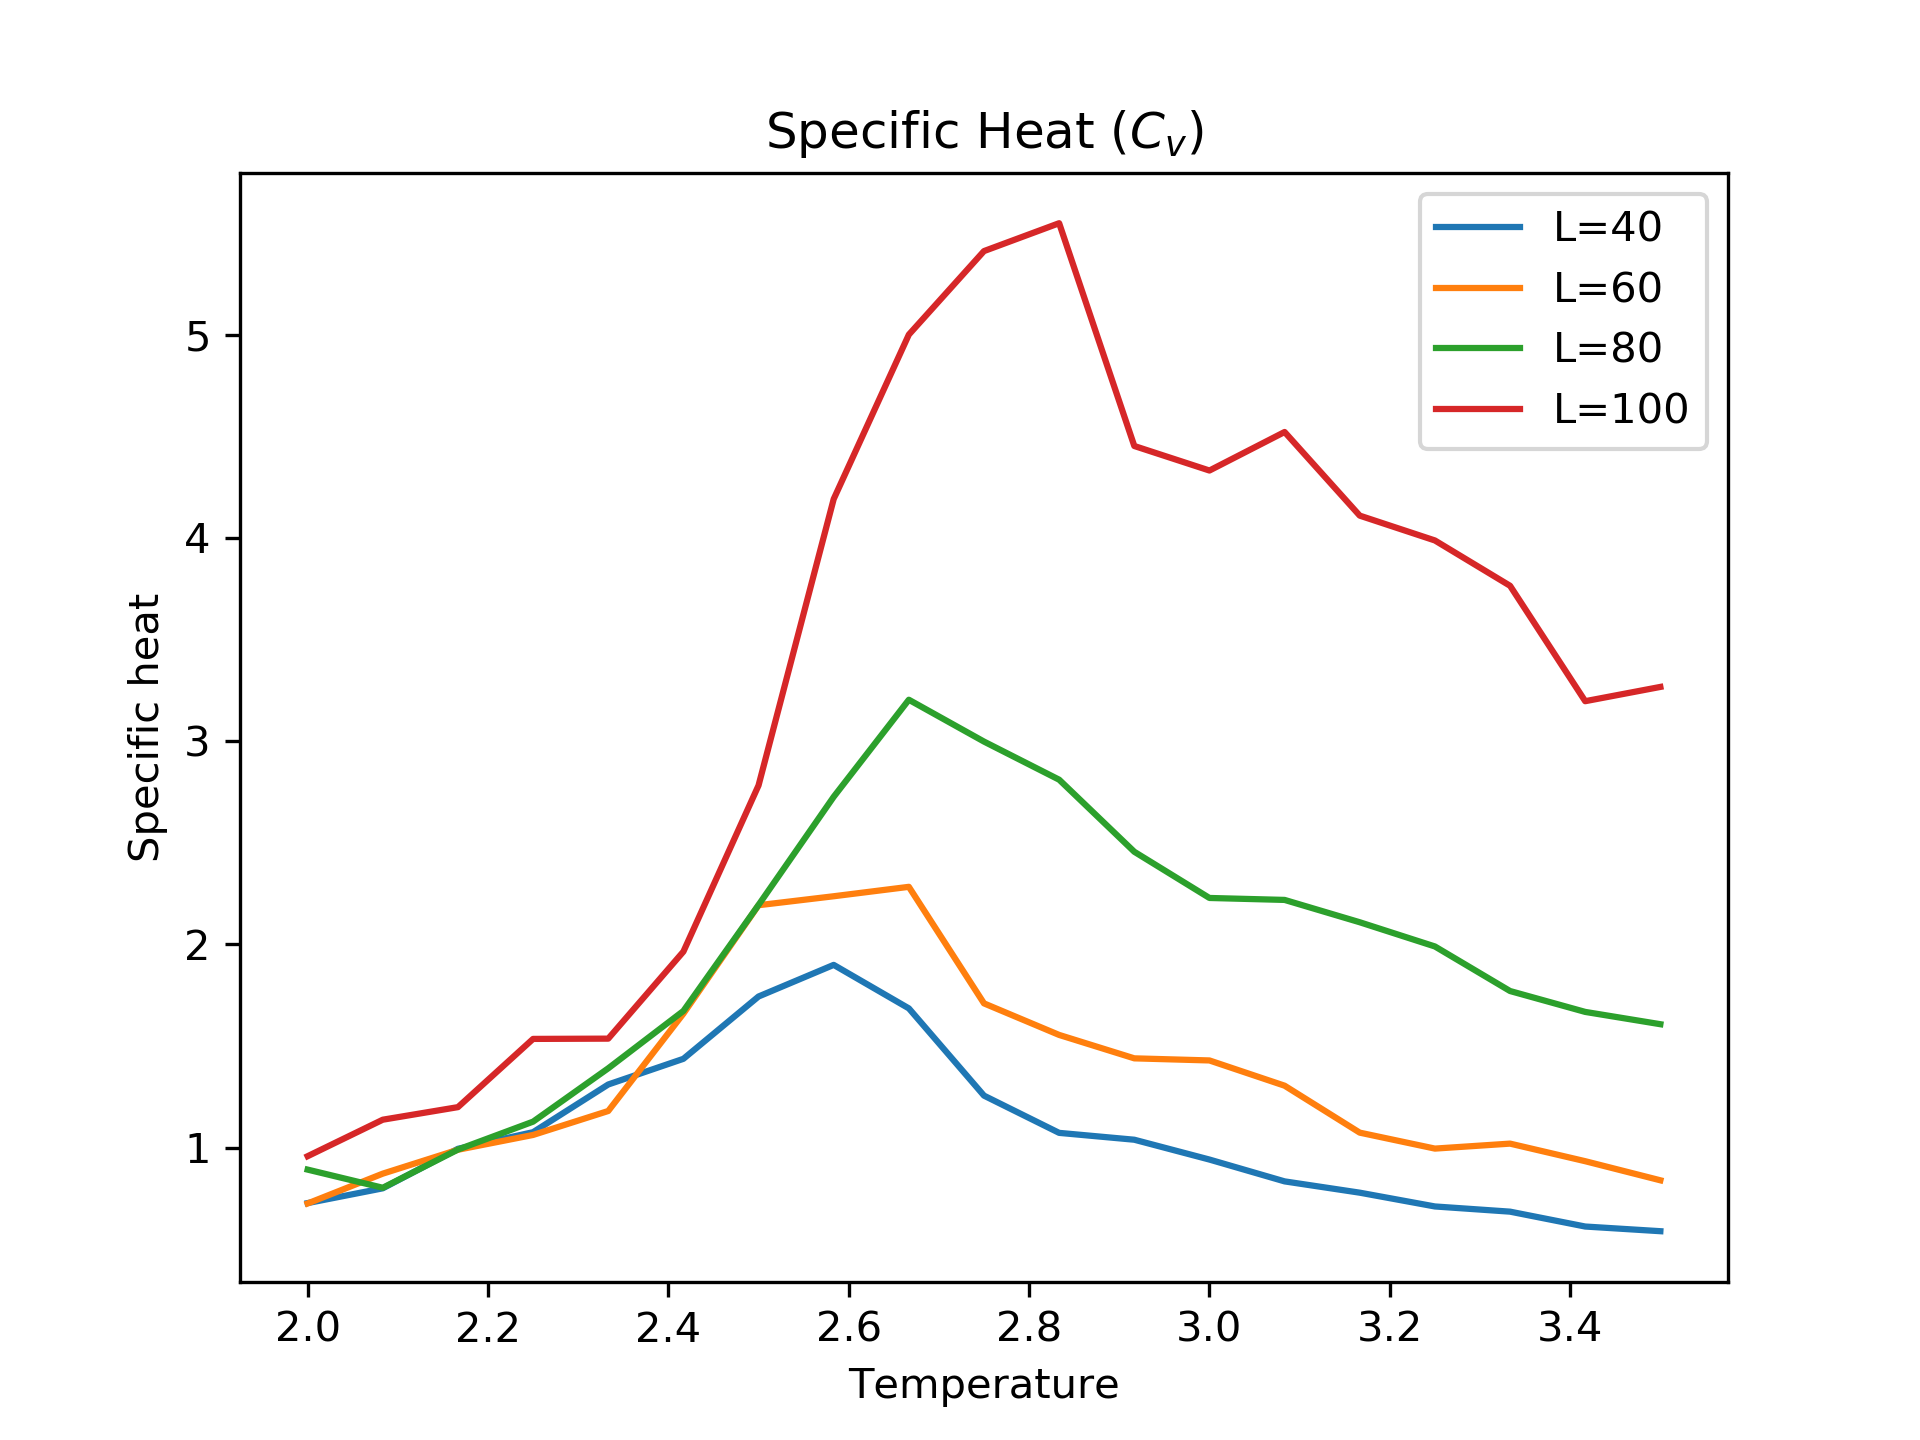
\includegraphics[width=250px]{./Plotting/Specific_heat.png}
				\caption{Specific Heat }
		\end{subfigure} \hfill %
		\begin{subfigure}{.5\textwidth}
				\centering
				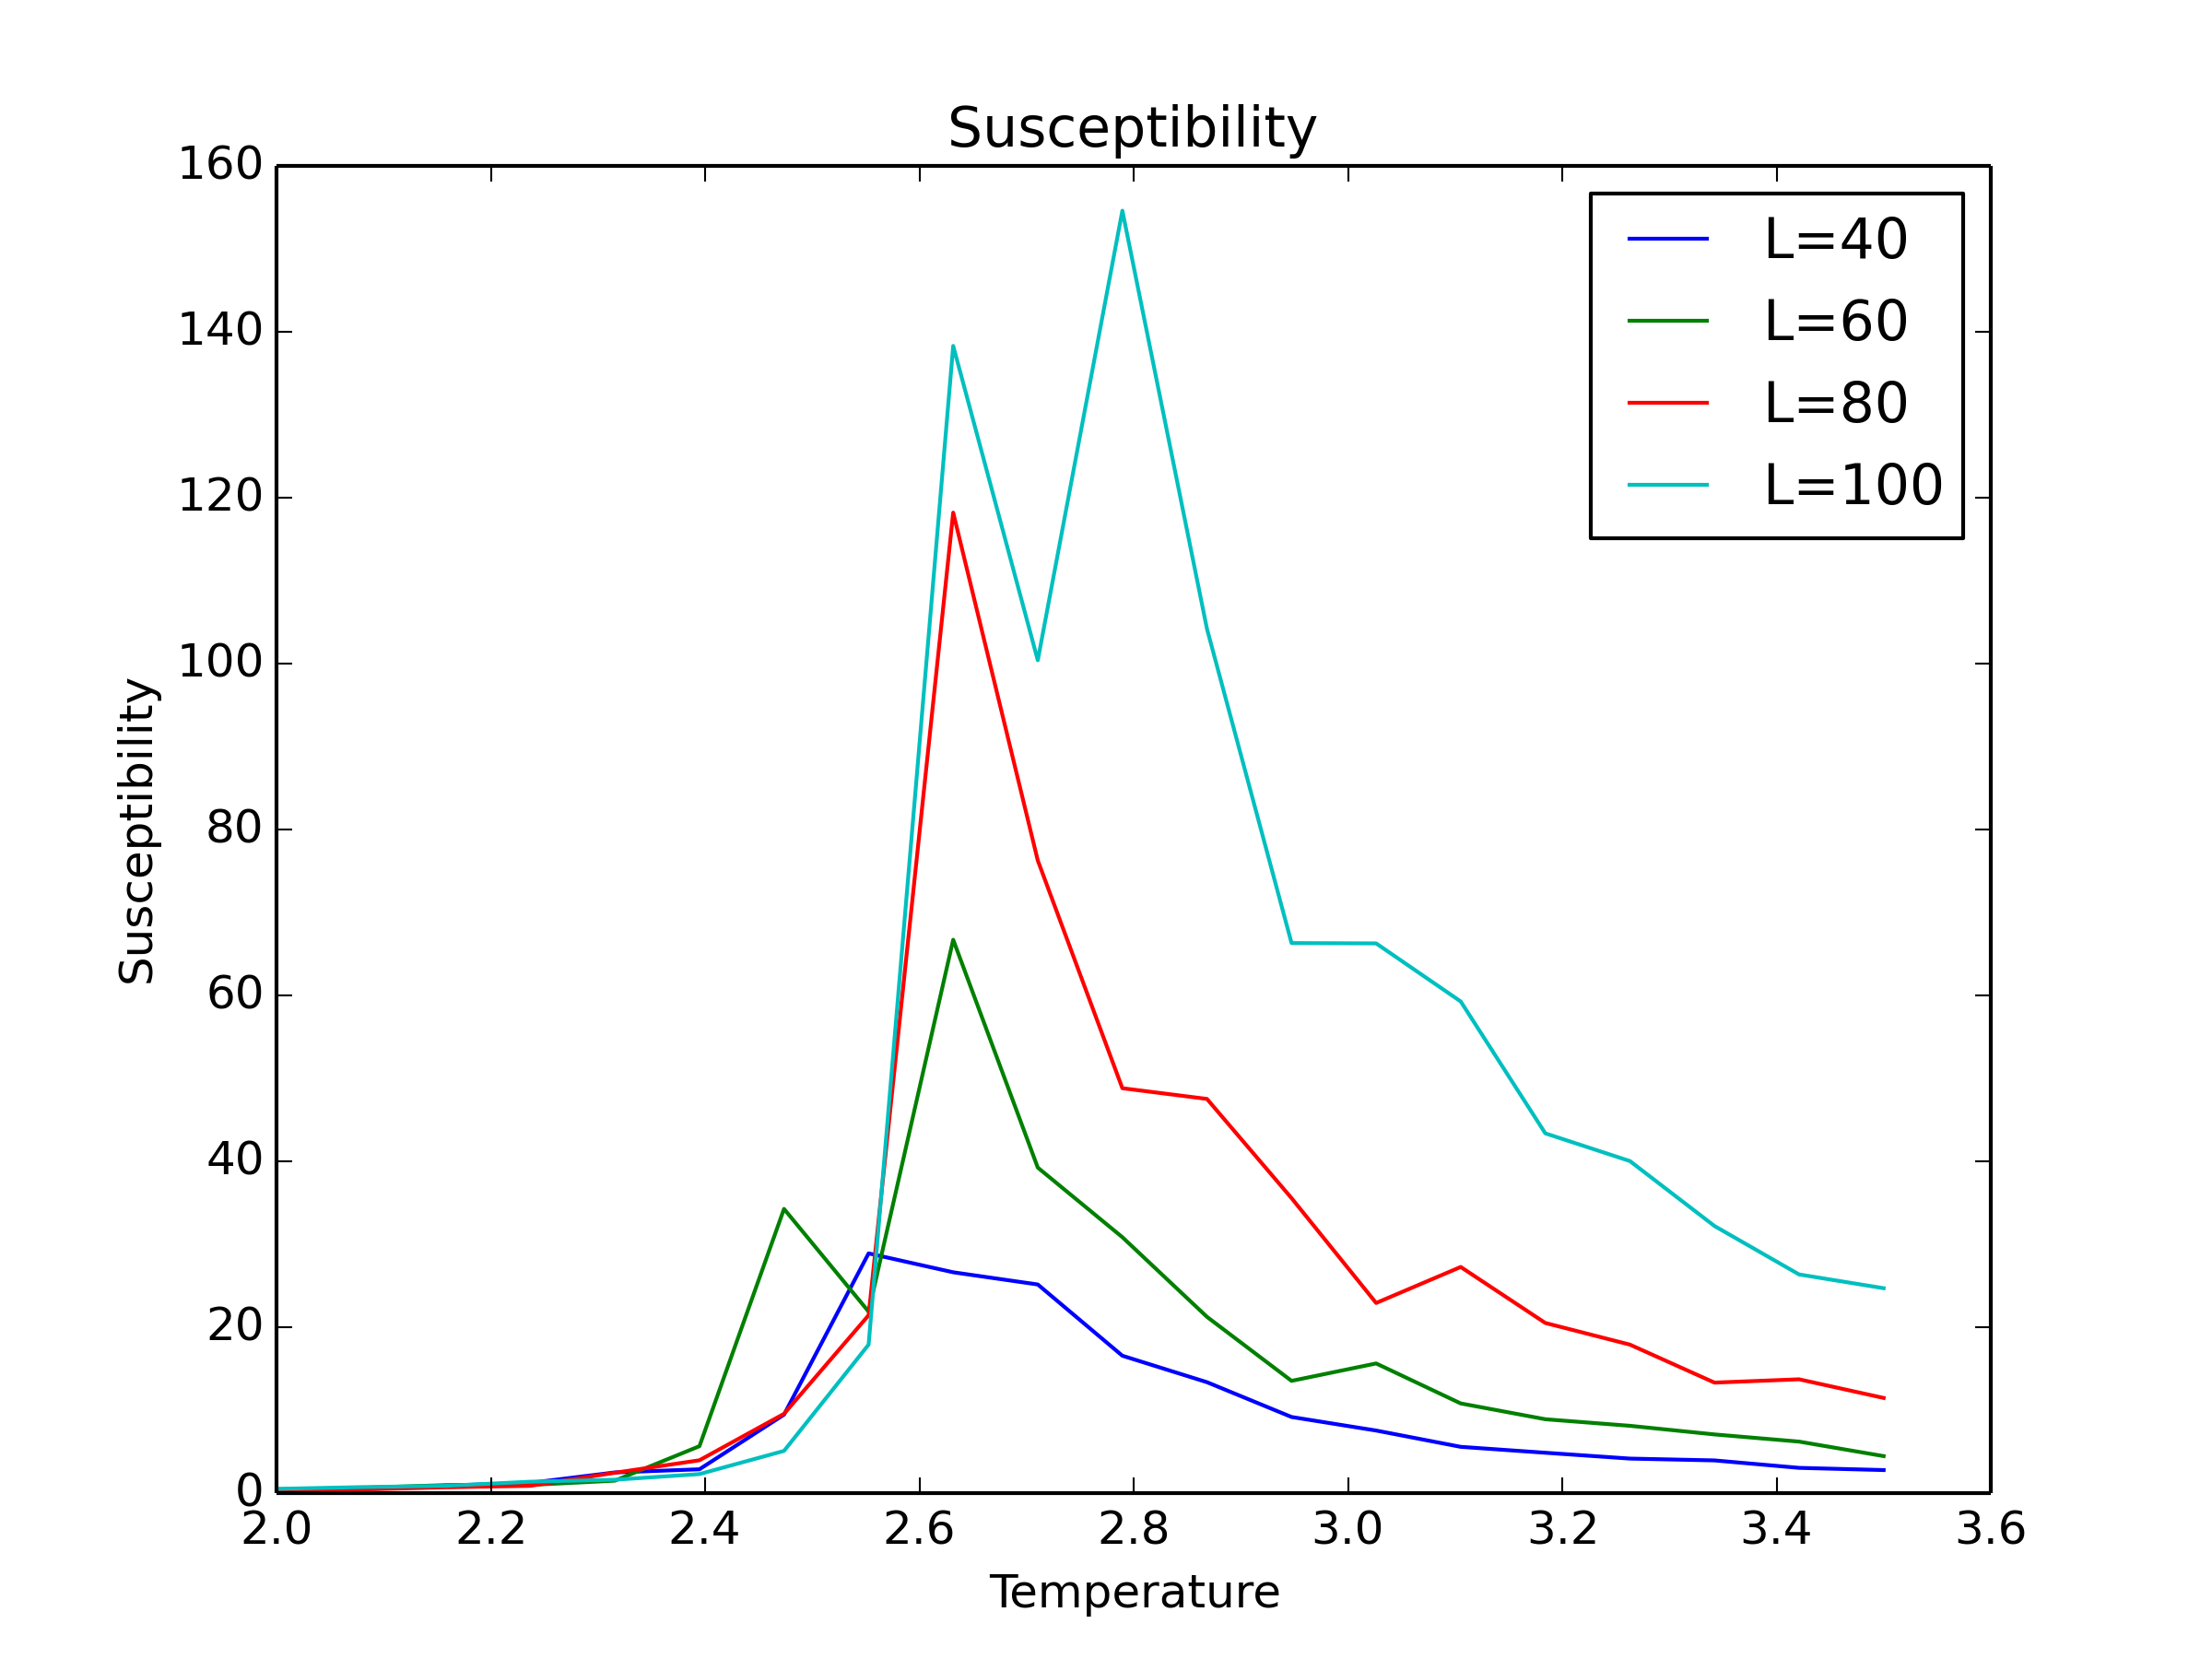
\includegraphics[width=250px]{./Plotting/Susceptibility.png}
				\caption{Susceptibility}
		\end{subfigure}\hfill}}
		\caption{: Specific heat and susceptibility as a function of temperature for different lattice sizes, L.}
		\label{fig:heat_susc}
		\end{figure}



\newpage
\section{Discussion}

	The numerical values for a 2x2 lattice is in good agreement with the analytical values. The mean magnetisation varies a lot in different calculations, because the magnetisation is heavily dependent on each single spin flip. While the energy dependence on each flip is the square value of the product of the neighboring spins, the magnetisation depends on the sum of all spins. This might be why we experience different values for the mean magnetisation in different calculations.\\

	% c)
	From Figure \ref{fig:steady_E} and \ref{fig:steady_M} we see that the energy stabilizes quite fast, at a low number of Monte Carlo cycles, at different energies, while the magnetization doesn't seem to stabilize at all.

 	Although the magnetisation never seems to stabilize for the initial random matix, as mentioned above, the magnetisation is more dependent on the spin configuration in the entire matrix, and will therefore not be as stable as the energy. Additionally, we have plotted the mean magnetisation for the highter temperature, while it might have been a better idea to plot the mean absolute magnetisation, like we did for the lower temperature.\\

	 When looking at Figure \ref{fig:flips} and Figure \ref{fig:flips_random} we can more easily see when the system stabilizes. In the beginning of the calculation, we can se that there is some change in number of flips which evens out fairly fast. When these plots even out we can consider that as a stable configuration since the number of accepted flips stays approximately the same. That means we have reached an equilibrium where the energy is as low as possible.

	 For this calculations, we calculated the spins inside a single Monte Carlo cycle, as opposed to for the stabilisation of the energy and magnetization, where we performed several different Monte Carlo cycles and compared those. A result of this is that the flip factor will not vary as much since the total number of flipped spins at the end of the loop does not differ that much. The flip facor could have varied more if we had calculated the flip factor of spins in different Monte Carlo loops.

	 From Figure \ref{fig:flips_random} we can see that for a random inital spin matrix the flip factor increases as the temperature increases. This indicates that the spins flip more often inside a single loop for higher temperatures.\\

	For the probability distribution, we have highlighted the mean energy when $T=2.4$. We chose not to do this for $T=1.0$, since this is clearly around $-800$. This is as expected, because for low temperatures none of the atoms will be recieving thermal energy from their suroundings. Therfore, the expected value for the system should be the lowest possible value (with some exceptions). For $T=2.4$, we can se that we have a nice Gaussian distribution around the mean energy value. When the temperature increases, some of the atoms will recieve energy from the surroundings and it will be more random how much energy each of the configurations will have. With this in mind, it is likley that we will have a distribution looking like this. We had some trouble calculating the variance of the energy, so this is not highlighted in the plot. Our expected values for the variance would mean that plotting the variance would take up around 60\% of the total area of the distribution.

	We used the function $interpolate.interp1d$ from SciPy in the plotting program $final_plot.py$ to find the temperature for the maximum value from the plots in Figure \ref{mean_E_M} and \ref{heat_susc}.

	The analytical value for the critical temperature is $2.269$. This is different from our simulated and extrapolated critical temperature for an infinite lattice, $2.78$. We can only assume that this is a consequence of a programming error, that could possibly also have caused our trouble with the variance above.

\section{Conclusion}
	Our results show that the temperature of the system has an effect on the physical values of the system, like the mean energy. Whether we start with random flips or not doesn't affect the values at all, which is as expected, because our measurements mostly happen after the system has reached equilibrium. We have also seen that the time it takes for the systems with different energies and spin starting points doesn't really vary a lot, and seem to stabilize at around $50 000$ Monte Carlo cycles. We do however see that when the temperature increases, the spins flip more often, resulting in higher energies, but similar magnetisation, up to the critical temperature.

	Studying the system further, we discover some discrepancies with expected results, such as the variance of the energy and magnetisation, following through to the magnetic susceptibility and the specific heat, meaning that we get an unexpectedly high extrapolated critical temperature for the phase change. This leads us to believe that our findings in this project are not precise enough to be comparable to other sources of information at the current time.

	Unfortunately, this project took a lot more work and therefore time to complete, meaning we did not have time to go further in depth in our methods to discover the error source.


\section{Appendix}
	\subsection{Degenerated Energies and Magnetization}

		When calculating the degenerate energies for a 2x2 lattice, we start with the equation $E_i=-J\sum\limits_{\left<kl\right>}^{2}s_ks_l$\\
		The case for all spins up looks like this:
		\begin{tabular}{c c}
			$\uparrow$ & $\uparrow$\\
			$\uparrow$ & $\uparrow$
		\end{tabular}\\

		The energy for this system is:
		\begin{flalign*}
			E_1 &= -J\sum\limits_{<kl>}^{2}s_k s_l\\
			&= -J((s_1 s_2+s_1 s_3)+(s_2 s_1+s_2s_4)+(s_3s_1+s_3s_4)+(s_4s_3+s_4s_2))\\
			&= -J((1+1) + (1+1) + (1+1) + (1+1))\\
			E_1 &= -8J
		\end{flalign*}
		In this calculation, we can see that the same interactions are counted twice. The reason for this is that the unit cell repeats itself to infinity in both x and y direction, which is our periodic boundary condition. Therefore the spin $s_1$ will interact with $s_2$ and $s_3$ inside of our unit cell, while $s_2$ and $s_3$ interact "outside" of the unit cell.

		The magnetisation is defined as:
		\begin{flalign*}
			M_i=\sum_{j=1}^{N} s_j
		\end{flalign*}
		which sums over all spins for a given configuration $i$. For the same spin configuration as above, this gives us:
		\begin{flalign*}
			M_i=\sum_{j=1}^{4} (1 + 1 + 1 +1) = 4
		\end{flalign*}

	\subsection{The Partition Function}
		When we known the values for all the degenerate energies we can calculate the value of the partition function.
		\begin{flalign*}
			&z = \sum\limits_{i=1}^{2^n}e^{-\beta E_i}\\
			&\text{For a 2x2-lattice, $n=4$.}\\
			&z = \sum\limits_{i=1}^{2^4}e^{-\beta E_i}\\
			&z = e^{-\beta E_1}+e^{-\beta E_2}+\hdots+e^{-\beta E_16}\\
			&z = e^{8 \beta J}+4e^{- \beta \cdot 0} + 2e^{-8 \beta J} + 4e^{-\beta \cdot 0} + 4e^{-\beta \cdot 0} + e^{8 \beta J}\\
			&z = 2e^{8 \beta J} + 2e^{-8 \beta J} + 12
		\end{flalign*}

	\subsection{Expectation Values for the Energy}
		The partition function is used to calculate the expectation value of the energy, $\left<E\right>$, and the terms involving energies that are 0 are omitted.

		\begin{flalign*}
			\left<E\right> &= \sum\limits_{i}^{2^n}\frac{E_i e^{-\beta E_i}}{z}\\
			&= \frac{-8Je^{8\beta J} +2\left(8Je^{-8 \beta J} \right) + \left(-8J\right)e^{8\beta J}} {2e^{8 \beta J} + 2e^{-8 \beta J} + 12}\\
			&= \frac{16J\left(e^{-8\beta J}- e^{8 \beta J} \right) }{2 {\left(e^{8 \beta J} + e^{-8 \beta J} + 6 \right)} }\\
			&= 8J \frac{e^{-8\beta J}- e^{8 \beta J}}{e^{8 \beta J} + e^{-8 \beta J} + 6}\\
			&= 8J \frac{sinh(8\beta J)}{cosh(8 \beta J) + 3}
		\end{flalign*}

		In order to calculate the variance, we need the expectation value of $E^2$.

		\begin{flalign*}
			\left<E^2\right> &= \sum\limits_{i}^{2^n}\frac{E_i^2 e^{-\beta E_i}}{z}\\
			&= \frac{64J^2e^{8\beta J} + 2\left(64J^2e^{-8\beta J}\right) + 64J^2e^{8\beta J}}{2e^{8 \beta J} + 2e^{-8 \beta J} + 12}\\
			&= \frac{128J^2e^{8\beta J} + 128J^2e^{-8\beta J}}{2e^{8 \beta J} + 2e^{-8 \beta J} + 12}\\
			&= 64J^2\frac{e^{8\beta J} + e^{-8\beta J}}{e^{8 \beta J} + e^{-8 \beta J} + 6}\\
			&= 64J^2 \frac{cosh(8\beta J)}{cosh(8\beta J) + 3}
		\end{flalign*}

	\subsection{Expectation Values for the Magnetization}
		The absolute value of the mean magnetisation is given by
		\begin{flalign*}
			\left<|M(T)|\right> = \frac{\sum \limits{_i^{2^4}} |M_i| e^{-\beta E_i}}{z}
		\end{flalign*}
		and can be calculated by using the values for the energy and the magnetisation from Table \ref{Tab: EogM}:

		\begin{flalign*}
			\left<|M(T)|\right> &= \frac{4e^{8\beta J} + 2\cdot4 + 0\cdot4 + 0\cdot2 + |-2|\cdot4 + |-4|e^{8\beta J}}{z}\\
			\left<|M(T)|\right> &= \frac{8e^{8\beta J} + 12}{2e^{8 \beta J} + 2e^{-8 \beta J} + 12} = \frac{4e^{8\beta J} + 8}{e^{8 \beta J} + e^{-8 \beta J} + 6}\\
			&= 8 \frac{e^{8\beta J} + 1}{cosh(8\beta J) + 3}
		\end{flalign*}

		We also have that
		\begin{flalign*}
			\left<|M(T)|^2\right> &=  \frac{\sum \limits{_i^{2^4}} |M_i^2| e^{-\beta E_i}}{z}\\
			\left<|M(T)|^2\right> &= \frac{32e^{8\beta J} + 32}{2e^{8 \beta J} + 2e^{-8 \beta J} + 12} = 16\frac{e^{8\beta J} + 1}{e^{8 \beta J} + e^{-8 \beta J} + 6}\\
			&= 16 \frac{e^{8\beta J}+ 1}{cosh(8\beta J) + 3}
		\end{flalign*}

	\subsection{Heat Capacity}
		We use the expectation values of the energy to calculate the variance:
		\begin{flalign*}
			\sigma^2_E &= \left<E^2\right> - \left<E\right>^2\\
		\end{flalign*}

		The heat capacity is defined as the variance divided by the energy and temperature squared.
		\begin{flalign*}
			C_v &= \frac{\sigma^2_E}{k_BT^2}\\
			&= \frac{64J^2}{k_bT^2}\left[\frac{cosh(8\beta J)}{cosh(8\beta J) + 3} \left(\frac{sinh(8\beta J)}{cosh(8 \beta J) + 3} \right)^2 \right]
		\end{flalign*}


	\subsection{Susceptibility}
		The variance of the absolute value of the mean magnetisation is given by:
		\begin{flalign*}
			\sigma_{M}^2 &= \left<|M(T)^2|\right> - \left<|M(T)|\right>^2\\
		\end{flalign*}

		We then calculate the susceptibility $\chi$, which is given by $\chi = \sigma_M^2/k_BT$.

		\begin{flalign*}
			\chi = \frac{1}{k_BT} \left[16 \frac{e^{8\beta J}+ 1}{cosh(8\beta J) + 3} - \left(  8 \frac{e^{8\beta J} + 1}{cosh(8\beta J) + 3}\right)^2 \right]
		\end{flalign*}

\section{Bibliography}

	\href{https://github.com/emmernme/MENA-Compfys/tree/master/Project4}{Link to our GitHub repository.}

	Morten Hjorth-Jensen, Lecture Notes FYS3150, chapter 12 and 13.

\end{document}
